%\documentclass[10pt]{article}
%\usepackage[utf8]{inputenc}
%\usepackage[T1]{fontenc}
%\usepackage{amsmath}
%\usepackage{amsfonts}
%\usepackage{amssymb}
%\usepackage{mhchem}
%\usepackage{stmaryrd}
%\usepackage{graphicx}
%\usepackage[export]{adjustbox}
%\graphicspath{ {./images/} }
%
%\begin{document}
%\textbackslash chapter\{Chapter 2\}

\section{CONCEPTOS BÁSICOS DE LOS SISTEMAS CONTROLADOS POR RETROALIMENTACIÓN SISO}
\section{INTRODUCCIÓN}
En este capítulo presentamos las propiedades básicas de los sistemas de retroalimentación de una sola entrada y salida sin considerar los problemas de robustez. En primer lugar, se define y discute la noción de margen de ganancia, margen de fase, ancho de banda y frecuencias cruzadas. Luego se explica por qué es tan importante disminuir el ancho de banda del controlador y en este sentido se define la ganancia de alta frecuencia.

Un controlador está diseñado para cumplir con las especificaciones de bucle cerrado deseadas, y se definen las especificaciones de dominio de tiempo y dominio de frecuencia. Aunque no existe una traducción uno a uno del dominio del tiempo a las especificaciones del dominio de la frecuencia, se proponen dos algoritmos que intentan cerrar la brecha.

Los beneficios de la retroalimentación para los sistemas de bucle abierto de fase no mínima son limitados en el sentido de que su ancho de banda tiene un límite superior. Por otro lado, si el bucle abierto es inestable, el ancho de banda tiene un límite inferior. Se dan ecuaciones y gráficos que relacionan estas limitaciones en función de los márgenes y las frecuencias cruzadas.

Finalmente, una sección está dedicada a ayudar al lector a adquirir habilidades en la configuración de bucles, a través de ejemplos y ejercicios.

\section{CARACTERÍSTICAS BÁSICAS DEL DOMINIO DE FRECUENCIA}
El sistema de retroalimentación considerado aquí se describe en la Fig. 2.1. Un ingeniero de control experimentado obtiene una excelente visión del comportamiento del sistema mirando el diagrama de Bode o Nichols del TF $L = P G H$ y el filtro $F$. El TF $L(s)$ se llama bucle abierto o transmisión de bucle, y el TF de cualquier entrada de comando, digamos $r$, a cualquier salida, digamos $y$, se llama TF de bucle cerrado de

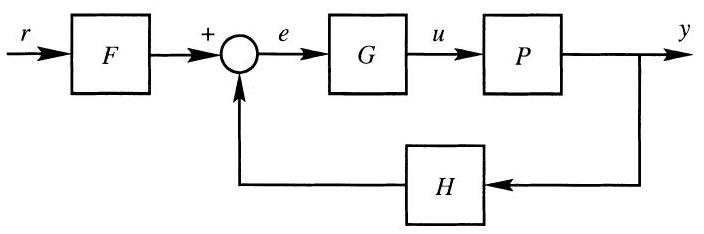
\includegraphics[max width=\textwidth]{2022_07_13_5539d24351f7cdb87589g-02}

Figura 2.1. Un sistema de retroalimentación de grado de libertad SISO 2

$r$ a $y$. Varios parámetros clave que gobiernan el comportamiento del sistema ahora están definidos y explicados.

\subsection{ESTABILIDAD RELATIVA, FRECUENCIA DE CRUCE Y ANCHO DE BANDA}
Un ejemplo de un diagrama de Nichols de un bucle abierto se muestra en la Fig. 2.2. Incluye 5 parámetros que caracterizan el sistema de bucle abierto y tienen un fuerte impacto en el comportamiento del sistema de circuito cerrado:

\begin{enumerate}
  \item Frecuencia cruzada o frecuencia de margen de fase, $\omega_{\phi}$ : es la frecuencia donde el bucle abierto es $0 d B,\left| L\left(j \omega_{\phi}\right)\right|=0 d B$.

  \item Margen de fase, $\phi$ : es la fase del bucle abierto en la frecuencia de cruce por encima de $-180^{\circ}, \phi=\arg L\left(j \omega_{\phi}\right)+180$.

  \item Frecuencia de margen de ganancia, $\omega_{M}$ : es la frecuencia donde $\arg L\left(j \omega_{M}\right)=-180^{\circ}$.

  \item Margen de ganancia, $M$ : es la distancia en $d B$ de $L\left(j \omega_{M}\right)$ desde el punto $-1$ en la gráfica de Nyquist $\left(0 d B,-180^{\circ}\right.$ en el gráfico de Nichols), $M=-20 \log \left| L\left(j \omega_{M}\right)\right|$.

  \item Ancho de banda, $\omega_{b}$ : varias definiciones de ancho de banda aparecen en la literatura, todas casi coinciden, elegimos aquí la frecuencia donde la amplitud del bucle cerrado es $-3 d B,\left|\frac{P G\left(j \omega_{b}\right)}{1+L\left(j \omega_{b}\right)}\right|=-3 d B$.

\end{enumerate}
En general, el margen de ganancia de estabilidad relativa y el margen de fase son cifras de mérito para dos aspectos importantes del sistema de circuito cerrado: (i) cuánta incertidumbre puede tolerar la planta y permanecer estable en el circuito cerrado, por ejemplo, si el margen de ganancia es de $10 \mathrm{~dB}$, el sistema puede tolerar un aumento de $10 \mathrm{~dB}$ en la ganancia sin perder la estabilidad del bucle cerrado; y (ii) pone un límite superior en la amplitud del TF de bucle cerrado desde el ruido del sensor hasta la salida de la planta, y un límite superior en la sensibilidad. Tener grandes márgenes de ganancia y márgenes de fase, implica la supresión de las resonancias de bucle cerrado en frecuencias alrededor de la frecuencia de ancho de banda $\omega_{b}$, pero surge un serio inconveniente en forma de un

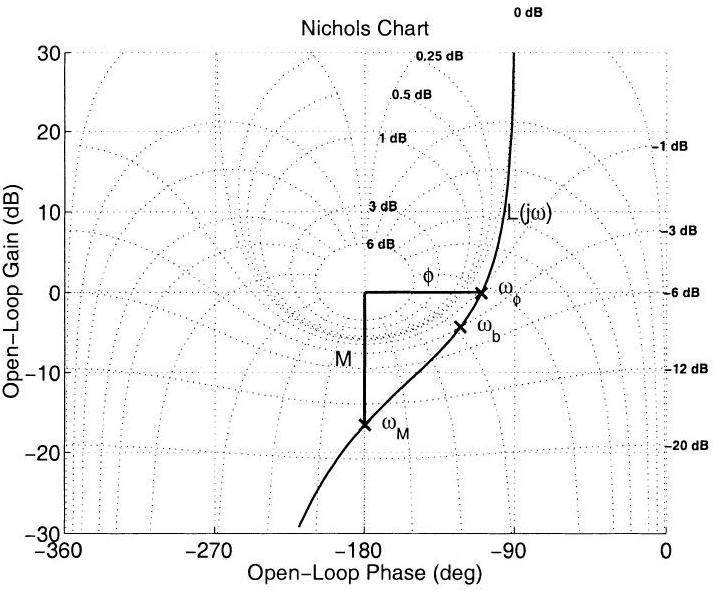
\includegraphics[max width=\textwidth]{2022_07_13_5539d24351f7cdb87589g-03}

Figura 2.2. Definición de margen de ganancia $M$, margen de fase $\phi$, frecuencia de cruce $\omega_{\phi}$, frecuencia de ancho de banda $\omega_{b}$, y frecuencia de margen de ganancia $\omega_{M}$, para el TF $L(s)$

Aumento de la respuesta al ruido del sensor en la entrada de la planta. Esto se ejemplifica en el siguiente ejemplo: Figuras 2.3-2.4 representan los gráficos de Nichols y Bode de 3 transmisiones de bucle, $L_{1}, L_{2}$ y $L_{3}$, con márgenes de $\left(130^{\circ}, 14 d B\right),\left(140^{\circ}, 12 d B\right)$ y $\left(150^{\circ}, 6.5 \mathrm{~dB}\right)$ respectivamente, y todos con la misma frecuencia de cruce. A partir de la Fig. $2.4$, el ruido del sensor en la entrada de la planta de $L_{1}$ es mucho mayor que el de $L_{2}$, que es mucho más alto que el de $L_{3}$. El ruido, cuyo espectro se encuentra en el rango de alta frecuencia, se amplifica en $L_{1}$ al orden de $ 6 d B$ más de lo que se amplifica en $L_{2}$ y en $ 16 d B$ más de lo que se amplifica en $L_{3}$.

Las definiciones anteriores no se mantienen si hay varias frecuencias cruzadas y / o varias frecuencias de margen de ganancia, en cuyo caso las cifras de mérito anteriores pueden ser engañosas. Los ejemplos se muestran en la Fig. 2.5.

\subsection{SISTEMAS CONDICIONALMENTE ESTABLES}
Los TF de bucle abierto pueden tener márgenes de ganancia positivos y negativos. Cualquier sistema práctico de bucle abierto tiene un margen de ganancia positivo, lo que significa que cuando el bucle se cierra, el sistema pierde estabilidad si la ganancia del bucle abierto aumenta demasiado. Si

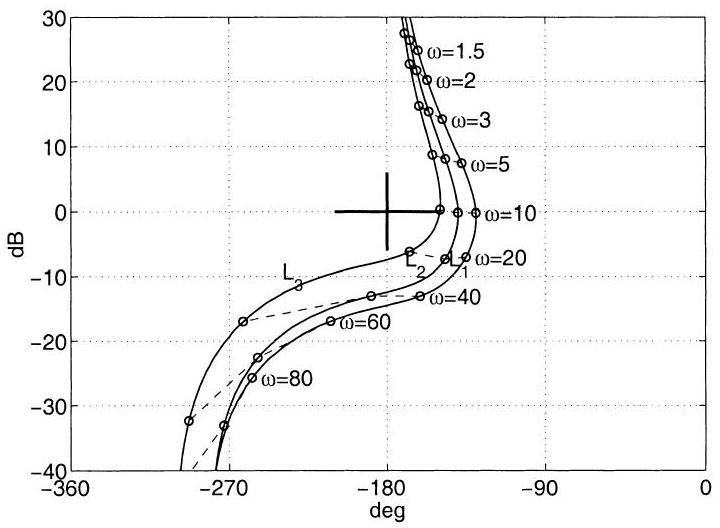
\includegraphics[max width=\textwidth]{2022_07_13_5539d24351f7cdb87589g-04}

Figura 2.3. Gráficos de Nichols de bucle abierto para $L_{1}, L_{2}$ y $L_{3}$, con casi las mismas características de baja frecuencia y la misma frecuencia cruzada, pero diferentes márgenes

Un sistema de bucle abierto tiene un margen de ganancia negativo, entonces el sistema en bucle cerrado pierde estabilidad si la ganancia de bucle abierto disminuye demasiado, y tales sistemas se llaman sistemas condicionalmente estables. La principal precaución práctica con tales sistemas es garantizar que durante la operación, la entrada de la planta no se sature, ya que tales sistemas pueden perder estabilidad fácilmente. La explicación matemática más simple de este fenómeno utiliza funciones de descripción y se basa en la suposición de que la saturación es equivalente a una disminución efectiva en la ganancia de bucle abierto (Gelb y Vander Velde, 1970). Otra explicación se basa en el criterio del círculo (Friedland 1996) que garantiza la estabilidad en el caso de saturación si $\left|\frac{1}{2} L(j \omega) /\left(1+\frac{1}{2} L(j \omega)\right)\right|<1$ para todas las frecuencias, una condición que nunca ocurre para los sistemas condicionalmente estables. Ejemplos de tales sistemas se muestran en la Fig. 2.6. Todos son inestables de bucle abierto, excepto el gráfico superior derecho, que es estable de bucle abierto.

\subsection{GANANCIA DE ALTA FRECUENCIA}
Como se mencionó en el Capítulo 1, uno de los factores que limita el ancho de banda del sistema (y, por lo tanto, limita el rendimiento del sistema) es el ruido del sensor en la entrada de la planta. Por ejemplo, veamos tres controladores para la planta $1 / s^{2}$, todos poseyendo\\

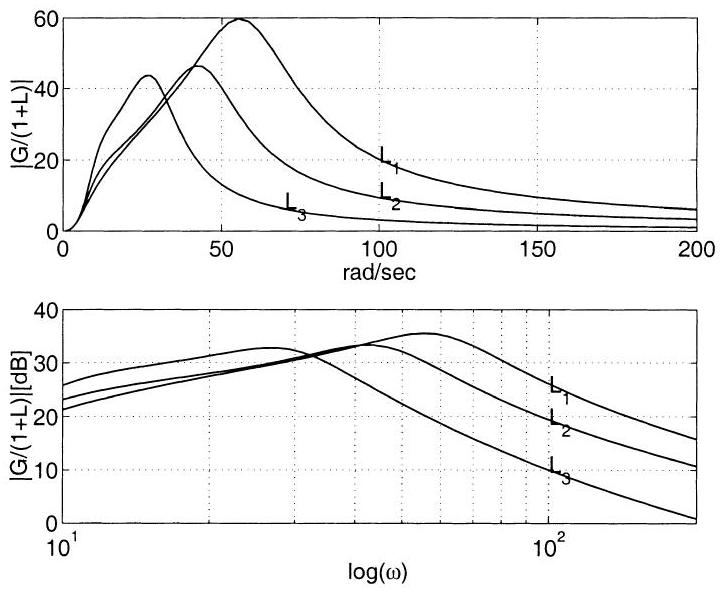
\includegraphics[max width=\textwidth]{2022_07_13_5539d24351f7cdb87589g-05}

Figura 2.4. TF desde el ruido del sensor hasta la entrada de la planta para la transmisión en bucle de la Fig. 2.3, gráfica superior en escala aritmética, inferior en escala logarítmica

casi el mismo comportamiento de bucle abierto de baja frecuencia y la misma frecuencia de cruce, pero con diferentes respuestas de alta frecuencia como se muestra en la Fig. 2.7. Los gráficos de los TF desde el ruido del sensor hasta la entrada de la planta, $G /(1+L)$, se dan en la Fig. 2.8. Claramente, si el espectro de ruido del sensor se concentra por encima de 80 $\mathrm{rad} / \mathrm{sec}$, el controlador $G_{3}$ es superior a los controladores $G_{1}, G_{2}$, y $G_{2}$ es superior a $G_{1}\left(G_{1}\right.$ amplifica las señales de ruido de alta frecuencia en $7 d B$ más que $G_{2}$ y en $20 \mathrm{~dB}$ más de $G_{3}$ ). Por lo tanto, una cifra importante de mérito para comparar dos controladores es: cuánto es el ruido del sensor amplificado en el rango de alta frecuencia por uno de los diseños en comparación con el otro. Entonces diremos que la ganancia de alta frecuencia de un diseño es mayor que la otra en $x d B^{\prime} s$, si su amplificación de ruido del sensor a altas frecuencias es mayor que el otro diseño por $x d B^{\prime} s$. Este tema fue tratado por Helton y Merino (1998) pp. 23-24 con respecto a la reducción del controlador y las compensaciones entre el ancho de banda y otras medidas de rendimiento.

Ejemplo: Dada la planta $P=10 / s^{2}$ y los dos controladores tales que sus TF de bucle abierto son $L_{1}$ y $L_{3}$ de Figs. 2.7-2.8. Sus actuaciones de circuito cerrado\\

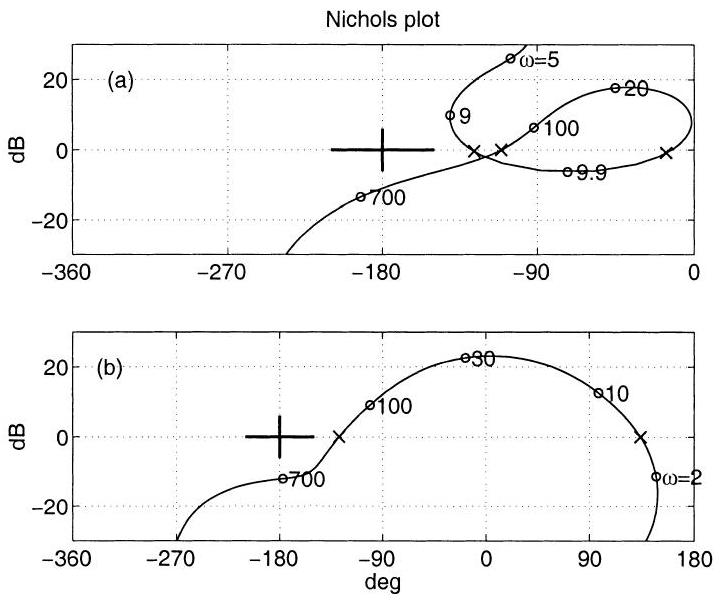
\includegraphics[max width=\textwidth]{2022_07_13_5539d24351f7cdb87589g-06}

Figura 2.5. a) un bucle abierto con 3 frecuencias cruzadas, marcadas con $\times$; (b) un bucle abierto con dos frecuencias cruzadas, marcadas $\times$

se espera que sean iguales porque $L_{1} \approx  L_{3}$ hasta la frecuencia de cruce. Ahora supongamos que el ruido del sensor es un ruido blanco coloreado pasándolo a través de un filtro de paso de banda $[40,300]^{1} \mathrm{rad} / \mathrm{sec}$. La Fig. $2.9$ describe la señal de entrada de la planta debido a ese ruido, la gráfica superior por $L_{1}$ y la inferior por $L_{3}$. Claramente, el RMS de la gráfica superior es al menos el doble que el de la gráfica inferior. Además, si la entrada de la planta se satura a $\pm 30$, el diseño cuyo bucle abierto es $L_{1}$ podría provocar inestabilidad, mientras que el diseño cuyo bucle abierto es de $L_{3}$ puede manejar perturbaciones y/o señales de seguimiento cuya respuesta en la entrada de la planta es de hasta $\pm 10(\pm 20$ para el ruido y $\pm 10$ para la señal de control).

\subsection{ANÁLISIS DE ESTABILIDAD USANDO GRÁFICOS DE NICHOLS}
Ahora desarrollamos el criterio de estabilidad gráfica utilizando el gráfico de Nichols en lugar de las técnicas estándar de plano complejo (diagramas de Bode o Nyquist), el

${ }^{1}$ El símbolo $[x, y]$ define un filtro de paso de banda con frecuencias de corte inferior y superior de $x$ y $y$ rad/seg respectivamente.\\

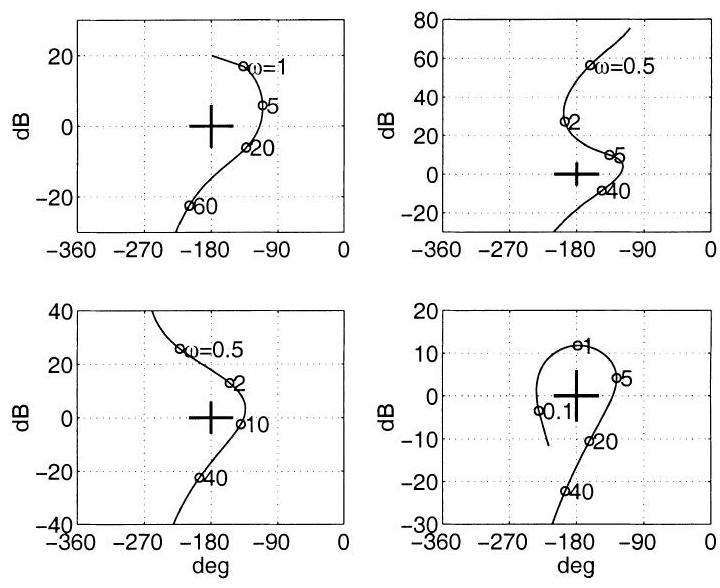
\includegraphics[max width=\textwidth]{2022_07_13_5539d24351f7cdb87589g-07}

Figura 2.6. Gráficos de Nichols de bucles abiertos condicionalmente estables TF's: Todos los sistemas de bucle abierto son inestables excepto la gráfica superior derecha que es estable de bucle abierto

La motivación es que el uso de gráficos de Nichols es una forma pictórica atractiva de diseñar y representar sistemas de retroalimentación. El desarrollo presentado aquí se basa en el trabajo de Cohen et al. (1994).

\subsection{SISTEMAS CONTINUOS}
Dado un sistema de retroalimentación cuyo bucle abierto, $L(s)$, es estrictamente apropiado, defina el contorno de Nyquist estándar, $\Gamma$, con dirección positiva en el sentido de las agujas del reloj, como el semicírculo cuyo radio es $R$ con $j hendiduras del eje \omega$-añadidas según sea necesario para dar cuenta de los polos imaginarios de $L(s)$. Se supone que $R$ es lo suficientemente grande como para incluir todos los polos inestables de $L(s)$. La multiplicidad total neta de estos polos se denota por $n$. La gráfica de Nyquist es la imagen de $L(s)$ en el plano complejo debido a $\Gamma$. El criterio de estabilidad de Nyquist para un sistema de retroalimentación es el siguiente:

TEOREMA $2.1$ El sistema de retroalimentación cuyo bucle abierto es $L(s)$ es estable si y sólo si la gráfica de Nyquist de $L(s)$ no interseca el punto $-1$ y lo rodea $n$ veces en sentido contrario a las agujas del reloj.

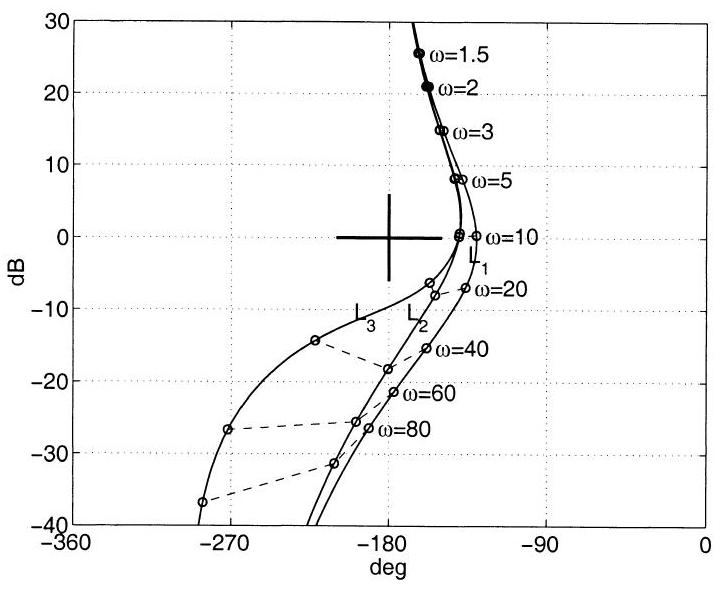
\includegraphics[max width=\textwidth]{2022_07_13_5539d24351f7cdb87589g-08}

Figura 2.7. Diferentes bucles abiertos con casi las mismas características de baja frecuencia y la misma frecuencia de cruce

Vidyasagar et al. (1988) presentó la siguiente simplificación del criterio de Nyquist. Dejando que $R_{0}$ sea el rayo $(-\infty,-1]$, se produce un cruce cuando la gráfica de Nyquist de $L(s)$ se cruza con $R_{0}$. Se dice que el cruce es positivo si la intersección es ascendente y negativo de lo contrario, ver Fig. 2.10.

TEOREMA $2.2$ El sistema de retroalimentación cuyo bucle abierto es $L(s)$ es estable si y sólo si la gráfica de Nyquist de $L(s)$ no interseca el punto $-1$ y lo rodea $n$ veces en sentido contrario a las agujas del reloj.

Nótese que en el teorema $2.2$ el rayo $R_{0}$ puede ser reemplazado por cualquier curva que conecte el punto $(-1,0)$ y el punto en $\infty$, bajo una definición adecuada de orientación de cruce.

\subsection{SISTEMAS DE TIEMPO DISCRETO}
Consideremos ahora un sistema de retroalimentación de datos muestreados con bucle abierto denotado por $L(z)$, que se supone que es estrictamente apropiado, mientras que $1+L(z)$ es correcto. El contorno de Nyquist estándar, $\Gamma$, encierra la región inestable del plano complejo $z$ y, por lo tanto, es el espacio fuera del círculo unidad con hendiduras en el\\

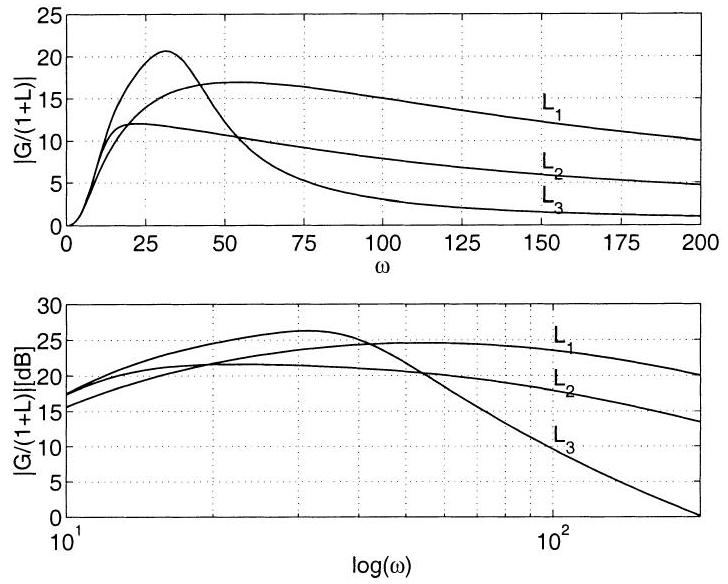
\includegraphics[max width=\textwidth]{2022_07_13_5539d24351f7cdb87589g-09}

Figura 2.8. TF desde el ruido del sensor hasta la entrada de la planta para la transmisión en bucle de la Fig, gráfica superior en escala aritmética, inferior en escala logarítmica

círculo unitario según sea necesario, para tener en cuenta polos de $L(z)$ en el círculo unitario. Sea $Z_{i}$ y $P_{i}$ denotan los ceros y polos de $1+L(z)$ dentro del círculo unitario, y $Z_{o}, P_{o}$ los ceros y polos de $1+L(z)$ fuera del círculo unitario, respectivamente. A partir del principio del argumento, el número de cercos del punto $-1$ hecho por la gráfica de Nyquist de $L(z)$ es $N$ donde $N=-\left(Z_{i}-P_{i}\right)$. Ahora, como $L(z)$ es estrictamente apropiado, el numerador y el denominador de $1+L(z)$ tienen el mismo orden polinómico, digamos $m$ y por lo tanto
$$
Z_{o}+Z_{i}=P_{o}+P_{i}=m,
$$
de ahí $N=Z_{o}-P_{o}$. La estabilidad está garantizada si y solo si $Z_{o}=0$, y por lo tanto si y solo si $N=-P_{o}$. El criterio de estabilidad de Nyquist para sistemas con bucle abierto TF $L(z)$, donde $n$ es el número total de polos de $L(z)$ fuera del contorno de Nyquist de tiempo discreto (incluyendo multiplicidad), es el siguiente:

TEOREMA $2.3$ El sistema de retroalimentación cuyo bucle abierto es $L(s)$ es estable si y sólo si la gráfica de Nyquist de $L(s)$ no interseca el punto $-1$ y lo rodea $n$ veces en sentido contrario a las agujas del reloj.\\

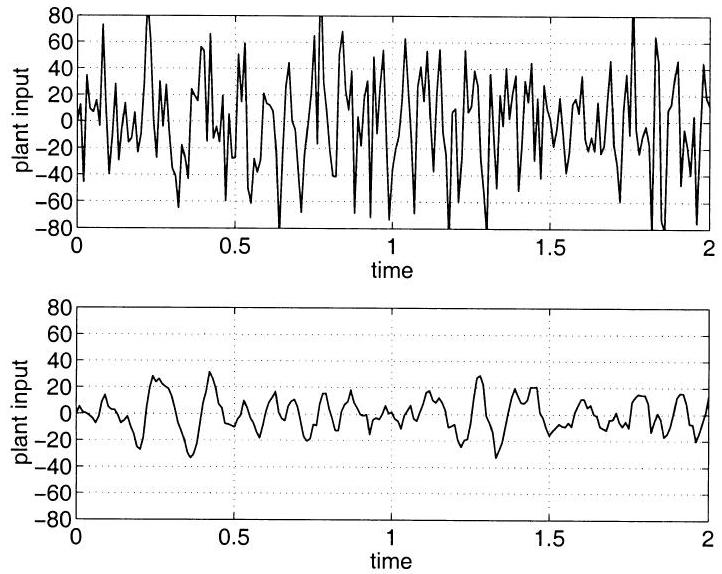
\includegraphics[max width=\textwidth]{2022_07_13_5539d24351f7cdb87589g-10}

Figura 2.9. Señal de entrada de planta para diferentes controladores con el mismo ancho de banda de bucle cerrado, gráfica superior por $L_{1}$, inferior por $L_{3}$

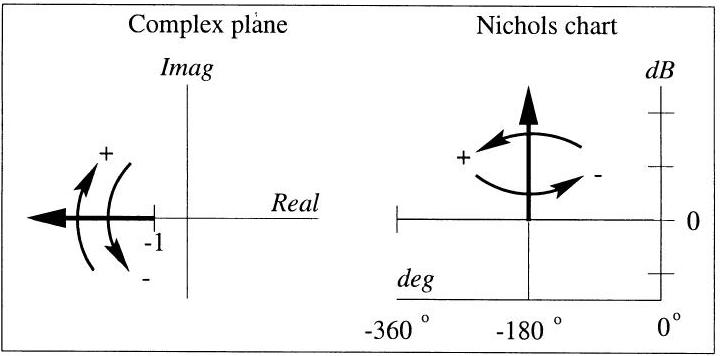
\includegraphics[max width=\textwidth]{2022_07_13_5539d24351f7cdb87589g-10(1)}

Figura 2.10. La noción de cruzar en $[d B, d e g]$ (derecha) y $[$ real, imag $]$ (izquierda), la flecha gruesa es el rayo $R_{0}$ Con las definiciones anteriores, la simplificación en Vidyasagar et al. (1988) puede ampliarse fácilmente al caso de los datos incluidos en la muestra. La noción de cruce es la misma que para el caso continuo.

TEOREMA $2.4$ El sistema de retroalimentación cuyo bucle abierto es $L(s)$ es estable si y sólo si la gráfica de Nyquist de $L(s)$ no interseca el punto $-1$ y lo rodea $n$ veces en sentido contrario a las agujas del reloj.

\subsection{ALGUNAS OBSERVACIONES SOBRE EL COMPLOT DE NYQUIST}
Se ha vuelto habitual en el diseño del sistema de control usar solo la mitad de la trama de Nyquist (solo la parte imaginaria positiva del contorno de Nyquist). Debido a la simetría conjugada, un cruce a unos $s_{0}$, implica otro cruce en su par conjugado complejo del mismo signo. Es decir, cada cruce de la mitad de la trama de Nyquist debe contarse dos veces. Usando la mitad de la gráfica de Nyquist, pueden ocurrir cruces no enteros que se convierten en un número entero cuando se cuentan dos veces. Tomemos por ejemplo $L(s)=10 /(s-1), L(0)$ cruza el rayo $R_{0} 1 / 2$ tiempo, pero cuando se cuenta dos veces los cruces se convierten en un número entero, 1 .

Supongamos que $L(s)$ no tiene polos en el eje imaginario, $1+L(s)$ no tiene ceros RHP, y $\omega_{\phi}$ denota la frecuencia de cruce más pequeña que es mayor que todas las frecuencias de cruce en el rayo $R_{0}$, entonces:

\begin{itemize}
  \item Si el número de polos RHP, $n$, es impar, $\arg L\left(j \omega_{\phi}\right)$ debe ser mayor que $-180^{\circ}$, y $L(0)$ debe estar en el rayo $R_{0}$, de lo contrario el número de cruces no puede ser un número impar.

  \item Si el número de polos RHP, $n$, es par y $| L(0)|>0 d B$, entonces $\arg L\left(j \omega_{\phi}\right)$ debe ser mayor que $-180^{\circ}$ y $L(0)$ no debe estar en el rayo $R_{0}$.

  \item Si $L(s)$ es estrictamente apropiado y $| L(0)|>0 d B$, entonces el signo de ganancia es positivo, es decir, en la siguiente representación $a_{0}>0$

\end{itemize}
$$
L(s)=\frac{a_{m} s^{m}+a_{m-1} s^{m-1}+\cdots+a_{0}}{s^{n}+b_{n-1} s^{n-1}+\cdots+b_{0}},
$$
siempre que no haya cancelación cero del polo RHP en $L(s)$ (Yaniv (1988) apéndice B).

Los TF de bucle abierto, $L(s)$, tales que $1+L(s)$ no tienen ceros RHP, tienen la siguiente propiedad muy importante: La fase de la frecuencia de cruce, $\arg L\left(j \omega_{\phi}\right)$, es negativa. Una clase grande para la cual esto es cierto se desarrolla en la sección 8. Esta clase incluye cualquier bucle abierto, $L(s)$, tal que $| L(0)|>1, L(s)$ es estrictamente apropiado y $L(s)$ tiene una frecuencia cruzada única.

\section{ESPECIFICACIONES DE LAZO CERRADO}
Considere el sistema de retroalimentación que se muestra en la Fig. 2.11. El TF $P(s)$ pertenece a un conjunto $\{P\}$ de plantas con incertidumbres, y los $G(s)$ y $F(s)$ del TF denotan el controlador y el prefiltro que se sintetizarán para cumplir con las especificaciones robustas de estabilidad y circuito cerrado. Especificaciones de bucle cerrado del sistema en

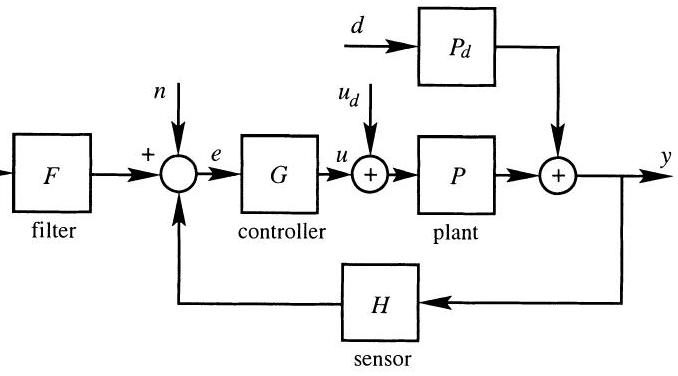
\includegraphics[max width=\textwidth]{2022_07_13_5539d24351f7cdb87589g-12}

Figura 2.11. Un sistema de retroalimentación SISO: $r, n, d$ y $u_{d}$ son entradas, $u$ y $y$

La Fig. $2.11$ se describe típicamente en el dominio del tiempo y/o el dominio de la frecuencia, abreviados como dominio $t$-domain y $\omega$-domain respectivamente. Las especificaciones del dominio t se relacionan con la respuesta del sistema en cualquier salida deseada debido a una entrada dada, mientras que las especificaciones del dominio $\omega$ son el dominio de frecuencia análogo a las especificaciones del dominio t. En la siguiente sección se describen estos tipos de especificación y se proporciona una traducción cuantitativa del dominio t al dominio $\omega$. La capacidad de traducir especificaciones de un dominio a otro es muy importante ya que todas las técnicas de diseño presentadas aquí están en el dominio $\omega$, mientras que una verdadera evaluación del rendimiento de un sistema de retroalimentación se realiza en el dominio t.

\subsection{ESPECIFICACIÓN DEL DOMINIO T}
Las especificaciones de bucle cerrado en el sistema en la Fig. $2.11$ se describen típicamente en términos de las señales de entrada y salida de la planta. Estos deben estar acotados de tal manera que el sistema funcione dentro de su región de trabajo y dé la respuesta de tiempo deseada. A continuación se presentan algunos ejemplos:

\begin{enumerate}
  \item La producción de la planta debe mantenerse cerca de cero (un sistema de regulación), las especificaciones pueden ser de la siguiente forma: para condiciones iniciales distintas de cero o perturbaciones dadas, la producción de la planta está limitada por una función de tiempo dada (ver Fig. 2.12a, b).

  \item La producción de la planta debe seguir una salida deseada dada (un servosistema) donde, debido a la incertidumbre de la planta, la salida deseada está limitada entre las funciones de tiempo superior e inferior (ver Fig. 2.12c). 3. La entrada de la planta, para un ruido de sensor dado y/o una perturbación dada y/o un comando de seguimiento dado, está limitada por una función de tiempo dada (a menudo para evitar la saturación, ver Fig. 2.12d).\\

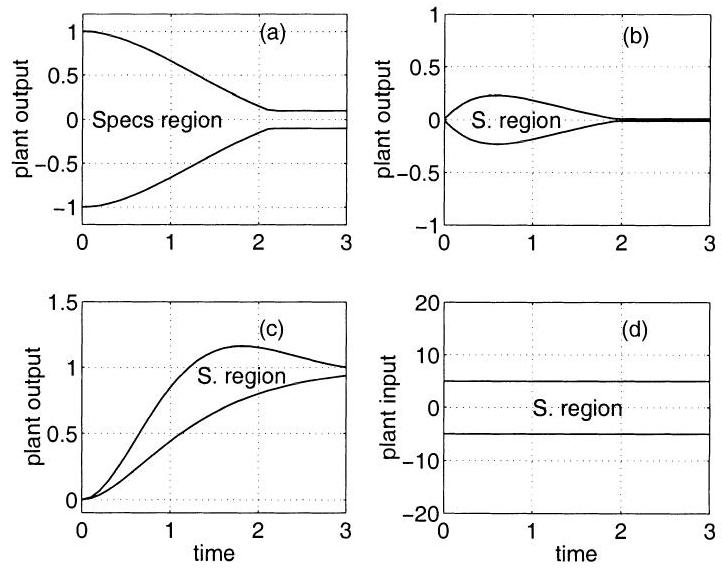
\includegraphics[max width=\textwidth]{2022_07_13_5539d24351f7cdb87589g-13}

\end{enumerate}
Figura 2.12. Ejemplos de especificaciones de dominio t: a), b) sobre la producción de la instalación para un conjunto determinado de condiciones iniciales; c) en la salida de la planta para un comando de paso; y d) sobre el insumo de la planta

Las especificaciones clásicas del dominio t, como el tiempo de subida de la respuesta escalonada, el tiempo de asentamiento, los errores de coeficiente de rebasamiento máximo (D'azzo y Houpis 1988) son casos especiales de los ejemplos anteriores. Los errores máximos de rebasamiento y coeficiente son, de hecho, especificaciones de dominio $\omega$-(D'azzo y Houpis 1988).

\section{2 $\omega$-DOMAIN SPECIFICATION}
Las especificaciones de bucle cerrado del sistema en la Fig. $2.11$ se describen típicamente en términos de desigualdades en los TF del sistema de algunas entradas a algunas salidas, estas son (usando la notación $L=P G H$ ):

\begin{enumerate}
  \item Rechazo de perturbación de la producción de la planta (Sensibilidad): para cualquier $P \in\{P\}$ el TF desde la perturbación en la salida de la planta hasta la salida de la planta está acotado por
\end{enumerate}
$$
\left|\frac{y}{d}\right|=\left|\frac{1}{1+L(j \omega)}\right|<\delta_{s}(\omega) .
$$

\begin{enumerate}
  \setcounter{enumi}{2}
  \item Rechazo de perturbación de entrada de planta: para cualquier $P \in\{P\}$ el TF de la perturbación en la entrada de la planta a la salida de la planta está limitado por
\end{enumerate}
$$
\left|\frac{y}{u_{d}}\right|=\left|\frac{P(j \omega)}{1+L(j \omega)}\right|<\delta_{p}(\omega) .
$$

\begin{enumerate}
  \setcounter{enumi}{3}
  \item Coincidencia del modelo: para cualquier $P \in\{P\}$ la distancia del TF de $r$ a $y$ del TF óptimo dado, $F_{m}(j \omega)$, está limitada por
\end{enumerate}
$$
\left|\frac{y}{r}-F_{m}\right|=\left|\frac{P G F(j \omega)}{1+L(j \omega)}-F_{m}(j \omega)\right|<\delta_{m}(\omega) .
$$

\begin{enumerate}
  \setcounter{enumi}{4}
  \item Seguimiento: para cualquier $P \in\{P\}$ la amplitud del TF de $r$ a $y$ está limitada por
\end{enumerate}
$$
\alpha(\omega) \leq\left|\frac{P G F(j \omega)}{1+L(j \omega)}\right| \leq \beta(\omega) .
$$

\begin{enumerate}
  \setcounter{enumi}{5}
  \item Rechazo de ruido: para cualquier $P \in\{P\}$ el TF desde la salida del sensor hasta la salida de la planta está limitado por
\end{enumerate}
$$
\left|\frac{y}{n}\right|=\left|\frac{P G(j \omega)}{1+L(j \omega)}\right|<\delta_{n}(\omega) .
$$

\begin{enumerate}
  \setcounter{enumi}{6}
  \item Esfuerzo de control: para cualquier $P \in\{P\}$ el TF desde la salida del sensor hasta la entrada de la planta está limitado por
\end{enumerate}
$$
\left|\frac{u}{n}\right|=\left|\frac{G(j \omega)}{1+L(j \omega)}\right|<\delta_{c}(\omega) .
$$
Para especificaciones $1-4$, la siguiente retención ( $H=1$ para simplificar)
$$
\begin{array}{ll}
\lim _{| G(j \omega)| \rightarrow \infty}\left|\frac{1}{1+L(j \omega)}\right|=0 \\
\lim _{| G(j \omega)| \rightarrow \infty}\left|\frac{P(j \omega)}{1+L(j \omega)}\right|=0 \\
\lim _{| G(j \omega)| \rightarrow \infty}\left|\frac{L F(j \omega)}{1+L(j \omega)}-F_{m}\right|_{F \equiv F_{m}}=0 \\
\lim _{| G(j \omega)| \rightarrow \infty} \frac{\max _{P(j \omega)} \frac{L F(j \omega)}{1+L(j \omega)}}{\min _{P(j \omega)} \frac{L F(j \omega)}{1+L(j \omega)}}=1 .
\end{array}
$$
Por lo tanto, a medida que aumenta la amplitud del controlador, la respuesta de salida de la planta a las perturbaciones disminuye y la sensibilidad de la producción de la planta a los comandos de seguimiento disminuye. Entonces diremos que las especificaciones son más estrictas. Por lo tanto, las especificaciones más estrictas requieren un mayor $ | G(j \omega)|$, que a su vez implica un bucle abierto más grande $L(j \omega)$, y por lo tanto una mayor frecuencia de cruce. Por lo tanto, las especificaciones más estrictas implican un mayor ancho de banda.

Ahora consideremos las especificaciones 5 y 6 . Un $| más grande G(j \omega)|$ aumenta la respuesta de entrada y salida de la planta al ruido del sensor, lo que sugiere un mayor $\delta_{n}(\omega)$ y $\delta_{c}(\omega)$ en un ancho de banda más amplio. Cualitativamente esto se puede explicar de la siguiente manera: El TF considerado en la especificación 5 es $L /(1+L)$ que es en general un filtro de paso bajo que opera en el ruido del sensor, con un ancho de banda de $\omega_{b}$ $\left(L\left(j \omega_{b}\right) \approx-3 d B\right)$. Un $| más grande G(j \omega)|$ provoca un aumento del ancho de banda, $\omega_{b}$, del TF de paso bajo del ruido a la salida de la planta, aumentando así la respuesta de ruido tanto en la salida de la planta como en la entrada. La misma explicación es válida para la especificación 6 porque $G /(1+L)=\frac{L / P}{1+L}$ y $P$ no es un parámetro de diseño. Por lo tanto, hay una compensación entre las especificaciones $ 1-4$ y 5,6. Un buen diseño de retroalimentación es aquel en el que las especificaciones $ 1-4$ están bien satisfechas sin hacer que las especificaciones del tipo 5,6 sean demasiado estrictas.

La ganancia de estabilidad relativa y los márgenes de fase son casos especiales de especificación 1 y 5 donde $\delta_{s}$ y $\delta_{n}$ son constantes. Se puede demostrar mediante aritmética simple que para $\delta_{s}=\gamma$ los márgenes de ganancia y fase son
$$
20 \log \left\{\frac{\gamma}{\gamma-1}\right\}[d B], 2 \sin ^{-1}\left\{\frac{1}{2 \gamma}\right\}[d e g]
$$
y para $\delta_{n}=\gamma$ los márgenes de ganancia y fase son
$$
20 \log \left\{\frac{\gamma+1}{\gamma}\right\}[d B], 2 \sin ^{-1}\left\{\frac{1}{2 \gamma}\right\}[d e g]
$$
La especificación de rechazo de perturbación 1 con constante $\delta_{s}$ limita la distancia del bucle abierto $L(s)$ evaluado en $L(j \omega)$ desde $-1$ en la gráfica de Nyquist $\left(0 d B,-180^{\circ}\right.$ en el gráfico de Nichols) colocando así un límite superior en la amplificación de la respuesta de salida de la planta a las perturbaciones en la salida de la planta,  en el dominio de la frecuencia. Como tal, es una especificación más atractiva que la ganancia relativa y los márgenes de fase (que teóricamente colocan el límite superior anterior solo en dos frecuencias discretas: $\omega_{\phi}$ y $\omega_{M}$ ). Lo mismo es cierto para la especificación 5 con una constante $\delta_{n}$. Pone un límite superior en el TF desde el ruido hasta la salida de la planta y, como tal, elimina los postes de bucle cerrado bajo amortiguación en el rango de frecuencia significativo del sistema.

\subsection{TRADUCCIÓN DE ESPECIFICACIONES DE T-DOMAIN A $\omega$-DOMAIN}
No hay una traducción uno a uno del dominio t propuesto a las especificaciones del dominio $\omega$-domain. Desde un punto de vista práctico, sin embargo, existen muy buenas traducciones, dos de las cuales se describen ahora. Desde nuestra experiencia, estas técnicas dan muy buenos resultados, pero si el diseñador no está satisfecho, puede iterar, por ejemplo, simplemente agregando ganancia en las frecuencias bajas (con modificaciones apropiadas de las frecuencias altas para satisfacer los márgenes especificados), hasta que se logren los resultados deseados.

También se recomienda relajar las especificaciones del dominio $\omega$-domain por encima de una cierta frecuencia, $\omega_{h}$, para satisfacer solo las especificaciones de ganancia y margen de fase. Esto es muy atractivo para reducir el esfuerzo de control con un impacto insignificante en el rendimiento del circuito cerrado. Las iteraciones en $\omega_{h}$ pueden ser necesarias, pero es muy fácil llevar a cabo y evaluar las compensaciones entre $\omega_{h}$, el esfuerzo de control y las especificaciones del dominio t.

\subsection{TÉCNICA BASADA EN MODELO}
Este método se basa en una estructura de modelo de planta y controlador asumida (se conoce el número de polos y ceros de la planta y el controlador). Por lo tanto, para una entrada dada, se puede calcular la estructura del modelo sobre la que se imponen las especificaciones. La idea es buscar los parámetros de los modelos de planta y controlador asumidos, y luego usar el máximo o mínimo de la amplitud del TF resultante en el eje $j \omega$ como la especificación de dominio $\omega$.

Ejemplo 1: Supongamos que la planta es un integrador simple $1 / s$, incrustado en una estructura de retroalimentación para lograr las siguientes especificaciones de dominio t de bucle cerrado: La producción de la planta para una perturbación escalonada en la salida de la planta debe estar limitada por las dos curvas de la Fig. 2.13a. Supongamos que la estructura del controlador es un polo simple, es decir, $G=k /(s+a)$. El primer paso es calcular la estructura del modelo de producción de la planta
$$
y(s)=\frac{1}{1+P G} \frac{1}{s}=\frac{1}{1+\frac{k}{s(s+a)}} \frac{1}{s}=\frac{s+a}{s^{2}+a s+k} .
$$
El segundo paso es buscar los $a$ y $k$ que satisfagan las especificaciones del dominio t. Este conjunto de salidas se denota por $\{y(s)\}$ en el dominio de frecuencia. El tercer paso es calcular la especificación $\omega$-domain, en este caso la especificación de sensibilidad, por
$$
\left|\frac{1 / s}{1+L(s)}\right|_{s=j \omega}=\max _{y \in\{y(j \omega)\}}|y(j \omega)| .
$$
Los resultados del cálculo anterior, para $a \in[1,8]$ y $k \in[2,12]$, se dan en la Fig. 2.13c. El sistema fue diseñado para satisfacer la especificación $\omega$-domain utilizando la técnica descrita en el Capítulo 3 , y el controlador resultante es $G=6 /(s+2.7)$. El diseño fue verificado por simulaciones y los resultados se presentan en la Fig. $2.13 \mathrm{c}, \mathrm{d}$. Claramente, se cumplen las especificaciones originales del dominio t y del dominio $\omega$ traducido. Pero lo que es más importante, las especificaciones del dominio t apenas se cumplen, lo que implica que la traducción al dominio $\omega$ no es conservadora.

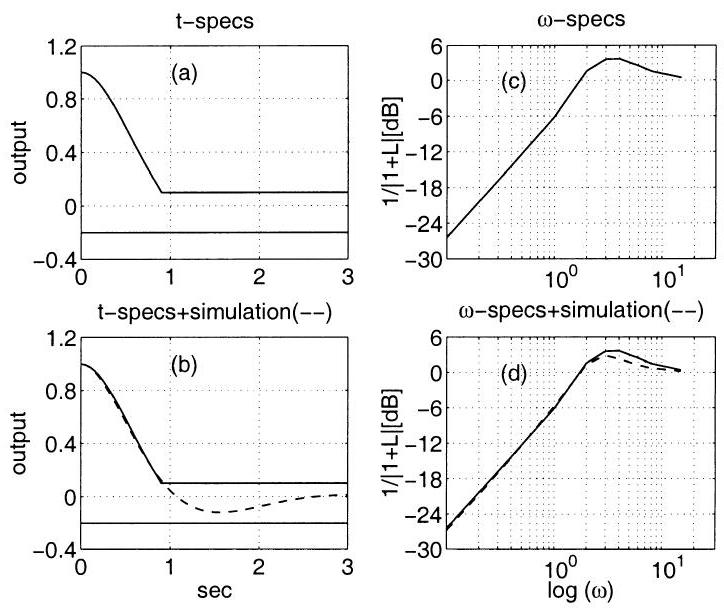
\includegraphics[max width=\textwidth]{2022_07_13_5539d24351f7cdb87589g-17}

Figura 2.13. Ejemplos de especificaciones de dominio t: a) la salida de una perturbación escalonada en la producción de la instalación deberá estar entre las curvas; b) simulaciones del dominio t (discontinuas) para una perturbación escalonada en la producción de la instalación; (c) $\omega$-domain specs sobre el TF de sensibilidad; d) la sensibilidad diseñada TF (discontinua)

Ejemplo 2: Supongamos que la planta es un integrador simple, $ 1 / s $, incrustado en una estructura de retroalimentación para lograr las siguientes especificaciones de dominio t de bucle cerrado: La salida de la planta para una perturbación escalonada en la entrada de la planta debe estar limitada por las dos curvas de la Fig. 2.14a. Se supone que el controlador incluye un integrador y un elemento principal, es decir, $G=k(s+a) / s(s+b)$. El primer paso es calcular la estructura del modelo de producción de la planta, que es
$$
y(s)=\frac{P}{1+P G} \frac{1}{s}=\frac{1}{1+\frac{k}{s} \frac{s+a}{s+b}} \frac{1}{s^{2}}=\frac{s+b}{s^{3}+s^{2} b+k s+k a} .
$$
El segundo paso es buscar los $a $ 's, $b$ 's y $k$ 's para los cuales se cumplen las especificaciones del dominio t. Este conjunto de salidas se denota por $\{y(s)\}$ en el dominio de frecuencia. El tercer paso es calcular la especificación $\omega$-domain, en este caso la especificación de sensibilidad
$$
\left|\frac{1 / s^{2}}{1+L(s)}\right|_{s=j \omega}=\max _{y \in\{y(j \omega)\}}|y(j \omega)| .
$$
Los resultados del cálculo anterior, para $a \in[0.5,2], b \in[2.5,9]$ y $k \in$ $[3.5,14]$, se dan en la Fig. 2.14c. El sistema fue diseñado para satisfacer la especificación $\omega$-domain, utilizando la técnica descrita en el Capítulo 3 , y el controlador resultante es $G=(7.4 s+6.6) /\left(s^{2}+4.3 s\right)$. El diseño fue verificado por simulaciones y los resultados se presentan en la Fig. $2.14 \mathrm{c}$,d. Claramente, se cumplen las especificaciones originales del dominio t y del dominio $\omega$-transferido.\\

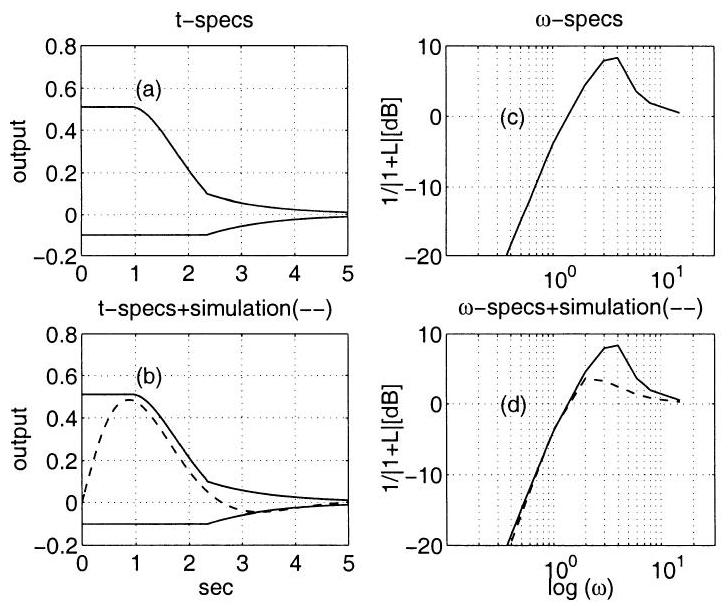
\includegraphics[max width=\textwidth]{2022_07_13_5539d24351f7cdb87589g-18}

Figura 2.14. Ejemplos de especificaciones de dominio t y dominio $\omega$: a) la salida de una perturbación escalonada deberá estar entre las curvas; b) simulaciones del dominio t (discontinuas) para una perturbación escalonada en la entrada de la instalación; (c) $\omega$-domain specs sobre el TF de sensibilidad; d) la sensibilidad diseñada TF (discontinua)

\subsection{TÉCNICA DE KRISHNAN Y CRUICKSHANKS}
Supongamos que las especificaciones del dominio t son de la forma
$$
|y(t)-m(t)|^{2} \leq v^{2}(t)
$$
donde $y(t)$ es la señal de bucle cerrado y $m(t), v(t)$ son funciones de tiempo especificadas. Es decir, $y(t)$ no debe desviarse de $m(t)$ en más de $v(t)$. Una condición más débil que esta es la siguiente:
$$
\int_{0}^{t}|y(t)-m(t)|^{2} \leq \int_{0}^{t} v^{2}(t), \forall t \geq 0,
$$
lo que significa que en lugar de que el límite superior de $|y(t)-m(t)|$ sea $v(t)$, la energía de la señal en el intervalo de tiempo $[0, t]$ está limitada por la energía de la señal $v(t)$ en el mismo intervalo (para cualquier $t$). Krishnan y Cruickshanks sugirieron usar esta condición más débil para la cual la condición suficiente en el dominio $\omega$-correspondiente a la desigualdad (2.2) es (Krishnan y Cruickshanks 1977)
$$
|y(j \omega)-m(j \omega)| \leq|v(j \omega)| .
$$
El principal inconveniente de esta técnica es que se utiliza una condición más débil, pero en general, es una alternativa razonable a la especificación original.

Ejemplo 3: Considere el sistema descrito en la Fig. $2.1$ y la especificación de dominio t de circuito cerrado en la salida de la planta $y(t)$
$$
a(t) \leq y(t) \leq b(t)
$$
donde $a(t), b(t)$ se dan en la Fig. 2.15a. Claramente, esta especificación es equivalente a
$$
|y(t)-m(t)| \leq v(t) ; m(t)=\frac{a+b}{2}, v(t)=\frac{b-a}{2},
$$
se muestra también en la Fig. 2.15a. Las especificaciones del dominio $\omega$-serán entonces
$$
\left|\frac{P G F r}{1+P G}-m(j \omega)\right| \leq|v(j \omega)|,
$$
que, para la elección del prefiltro tal que $F r=m(s)$, es la especificación de sensibilidad de dominio $\omega$-
$$
\left|\frac{m(j \omega)}{1+L}\right| \leq|v(j \omega)|, L=P G .
$$
Las amplitudes de $m(j \omega) \omega$ y $v(j \omega) \omega$ se muestran en la Fig. 2.15c en lugar de $m(j \omega)$ y $v(j \omega)$, debido a la conveniencia de trazar los gráficos. Como se argumenta en el capítulo 3, es importante relajar las especificaciones a altas frecuencias para ahorrar ancho de banda. La curva discontinua en la Fig. 2.15c son las especificaciones relajadas de $|v(j \omega) \omega|$ utilizadas para el diseño. Las simulaciones en el dominio del tiempo para $G=35 /(s+17.5)$ se muestran en la Fig. $2.15 \mathrm{~b}$; claramente las especificaciones del dominio t se cumplen excepto cerca de $t=0$ (Fig. 2.15d), la razón es la relajación de la especificación $|v(j \omega)|$ a frecuencias más altas.

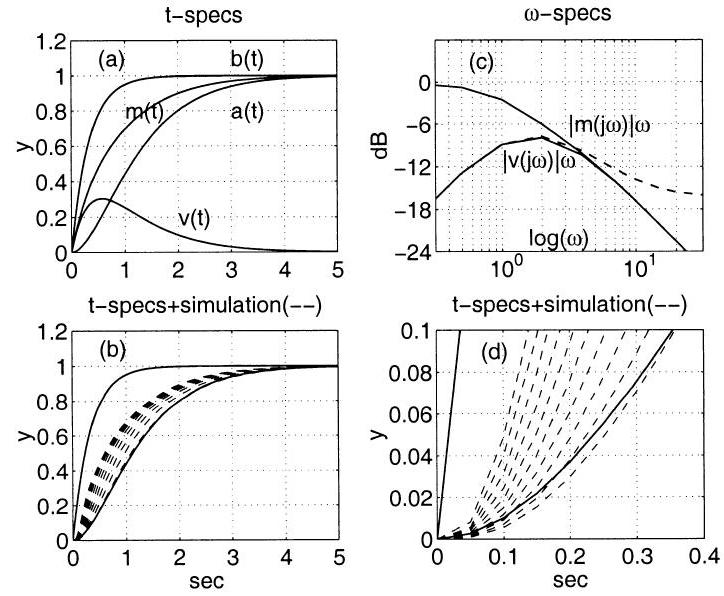
\includegraphics[max width=\textwidth]{2022_07_13_5539d24351f7cdb87589g-20}

Figura 2.15. Ejemplos de especificaciones de dominio t, (a) la salida de la planta para un comando de seguimiento de pasos debe estar entre las curvas $a(t), b(t)\left(m(t)=\frac{a+b}{2}\right.$ y $\left.v=\frac{a-b}{2}\right) ;(\mathrm{b}) \mathrm{t}$-domain simulations (discontinuo) para toda incertidumbre de la planta donde $F r=m(s) ;$ (c) $\omega$-especificaciones de sensibilidad de dominio,  La curva discontinua es el verdadero $|v \omega|$ utilizado para el diseño; (d) Simulación de dominio t cerca de $t=0$

\section{LIMITACIONES DE RENDIMIENTO DE NMP O SISTEMAS INESTABLES}
Las plantas de NMP son aquellas cuyo modelo incluye uno o más ceros RHP y / o retardo puro (el muestreo incluye inherentemente el retraso, por lo tanto, los sistemas de retroalimentación que incluyen muestreo también son NMP). Un ejemplo bien conocido es el péndulo invertido en un carro (Kailath 1980) para el cual es fácil explicar el fenómeno NMP: Si él / ella quiere mover la punta del péndulo hacia la derecha, el carro primero tiene que moverse hacia la izquierda para dejar que la punta caiga hacia la derecha y luego el carro se conduce hacia la derecha. La punta se moverá ligeramente hacia la izquierda y luego hacia la derecha. Por lo tanto, tomará más tiempo llevar la punta a un lugar deseado a la derecha en comparación con una planta que no tiene que moverse primero hacia la izquierda.

La frecuencia de cruce de bucle abierto, $\omega_{\phi}$, de un sistema NMP tiene un límite superior, por lo tanto, la amplitud de la transmisión de bucle a frecuencias por debajo de la frecuencia de cruce también está acotada. ${ }^{2}$ La razón se debe a las relaciones fase-amplitud de Bode. En los sistemas de fase mínima, se puede dar forma al bucle abierto con lead-lags, lag-leads, etc. de tal manera que se pueda lograr cualquier frecuencia de cruce deseada. Sin embargo, para las plantas de NMP, la frecuencia de cruce de transmisión de bucle está acotada (ver sección 8. para más explicaciones y fórmulas), y la ganancia de bucle a bajas frecuencias está acotada. Por ejemplo, si la frecuencia de cruce de un sistema que se comporta como $1 / s^{2}$ en bucle abierto a bajas frecuencias, es $10 \mathrm{rad} / \mathrm{sec}$, su ganancia de transmisión de bucle en $\omega=1$ no puede exceder $40 \mathrm{~dB}$. Por lo tanto, los beneficios de la retroalimentación para las plantas NMP son limitados en el sentido de que no se pueden lograr especificaciones de circuito cerrado utilizando un controlador LTI. Estas limitaciones dependen de los siguientes parámetros: el polo RHP y las ubicaciones cero, margen de ganancia, margen de fase y retardo de bucle abierto. Ahora sigue una discusión cuantitativa.

\subsection{PLANTAS ESTABLES}
Cualquier TF estable de bucle abierto, $L(s)$, se puede factorizar únicamente en $L(s)=$ $L_{M}(s) A(s)$ donde $L_{M}(s)$ es fase mínima (estable y no tiene RHP cero) y $A(s)$ un TF de paso completo (estable y $| A(j \omega)|=1$ para todos $\omega$ ), por ejemplo
$$
L(s)=\frac{s-1}{(s+2)(s+3)}=\overbrace{\frac{s+1}{(s+2)(s+3)}}^{\frac{1-s}{s+1}} .
$$
Basado en la relación de Bode entre la amplitud y la fase de una TF de fase mínima (Bode 1945, Horowitz 1963) si la fase de una TF estable de fase mínima en un amplio rango de frecuencia se fija en, digamos $\phi[\mathrm{deg}]$, entonces dentro de ese rango de frecuencia puede ser aproximada por el TF $k / s^{\phi / 90}$ (es equivalente a pedir que la gráfica de amplitud de Bode tenga una pendiente fija en un amplio rango de frecuencia). Añadiendo esta aproximación al criterio práctico de que el ancho de banda del controlador debe estar acotado, hacemos la siguiente suposición que se satisface en gran medida en sistemas de retroalimentación realistas y será

${ }^{2}$ Cierto en general, pero a una sola frecuencia podemos lograr, teóricamente, cualquier ganancia de bucle abierto usando osciladores de la forma $\frac{1}{s^{2}+\omega_{n}^{2}}$ como parte del controlador verificado numéricamente en la secuela (ver también Sidi (1997) y Horowitz y Sidi (1972)):

SUPUESTO $2.1$ Entre la frecuencia cruzada, $\omega_{\phi}$, y la frecuencia de margen de ganancia, $\omega_{M}$, la fase mínima $T F, L_{M}(s)$, puede aproximarse por
$$
L_{M}(s) \approx \frac{k}{s^{2 \alpha}} .
$$
Bajo el supuesto 2.1, si $L(s)$ incluye un solo RHP cero a $a$, entonces $L(s)=$ $L_{M}(s) \frac{a-s}{a+s}$ y por lo tanto
$$
\arg L(j \omega)=-\alpha \pi-2 \tan ^{-1}(\omega / a) ; \quad \omega_{\phi} \leq \omega \leq \omega_{M},
$$
que rinde para el margen de fase $\phi$, la frecuencia cruzada $\omega_{\phi}$ y la frecuencia de margen de ganancia $\omega_{M}$
$$
\begin{gathered}
\omega_{a \phi} \stackrel{\text { def }}{=} \frac{\omega_{\phi}}{a}=\tan \left\{\frac{(1-\alpha) \pi-\phi}{2}\right\} \\
\omega_{a M} \stackrel{\text { def }}{=} \frac{\omega_{M}}{a}=\tan \left\{\frac{(1-\alpha) \pi}{2}\right\} .
\end{gathered}
$$
A partir de las ecuaciones $(2.4,2.5)$ y la suposición 2.1, el margen de ganancia, denotado por $M$, es
$$
M=\left[\frac{\omega_{a M}}{\omega_{a \phi}}\right]^{2 \alpha}=\left[\frac{\tan \frac{\alpha \pi+\phi}{2}}{\tan \frac{\alpha \pi}{2}}\right]^{2 \alpha} .
$$
También a partir de las ecuaciones $(2.4,2.5)$ y la ecuación (2.6) se pueden calcular las relaciones entre el margen de ganancia, el margen de fase, la frecuencia cruzada y $\alpha$ y se muestran en la Fig. 2.16.

Ejemplo: Dada una planta con un solo RHP cero en $a=3$, por ejemplo
$$
P(s)=\frac{1}{s} \frac{3-s}{8+s}
$$
luego para el margen de fase $40^{\circ}$ y el margen de ganancia $M=10 d B$ (ver Fig. 2.16),
$$
\alpha=0.61, \quad \omega_{a \phi}=0.275, \quad \omega_{\phi}=a \times \omega_{a \phi}=3 \times 0.275=0.825
$$
y por ecuación (2.6)
$$
\omega_{M}=\frac{\log _{10} M}{2 \alpha} \times \omega_{\phi}=2.6 \times 0.875=2.8 .
$$
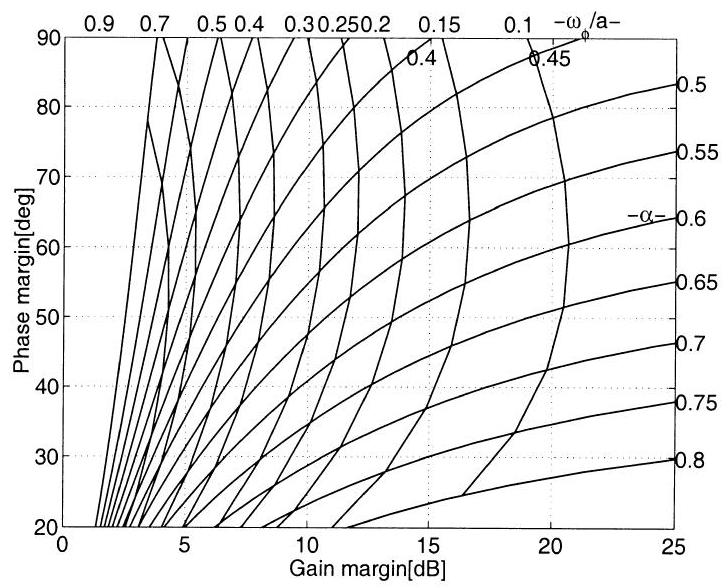
\includegraphics[max width=\textwidth]{2022_07_13_5539d24351f7cdb87589g-23}

Figura 2.16. Margen de fase vs. margen de ganancia para diferentes valores de $\alpha$ y $\omega_{\phi} / a$

Usando la forma de bucle tratando de maximizar $\omega_{\phi}$ para la especificación $|1+L(j \omega)|>$ $-3.5 d B$ (que conservan la misma ganancia y márgenes de fase) da
$$
L(s)=\frac{2.8 s^{2}+7.8 s+5.5}{s^{2}+3.5 s+0.67} P(s)
$$
cuyo TF se muestra en la Fig. 2.17. Su frecuencia cruzada es $0.93 \mathrm{rad} / \mathrm{sec}$, que es mayor que el valor estimado basado en la suposición $2.1$ por $12 \%$. Tenga en cuenta que el precio de este pequeño aumento es un aumento de $ 150 \%$ en $ \ omega_ {M}$ y, por lo tanto, un aumento muy grande en la amplificación de ruido en la entrada de la planta y en la frecuencia de muestreo mínima requerida en caso de implementación digital.

\subsection{EXTENSIÓN A VARIOS CEROS RHP Y/O RETRASO}
Plantas NMP con solo ceros RHP reales: Se puede lograr una estimación razonable de la relación entre margen de ganancia, margen de fase y frecuencia cruzada reemplazando los ceros RHP por un cero RHP único equivalente cuya fase es la aproximación de primer orden de los ceros RHP originales. Una fórmula simple es: para los ceros RHP ubicados en $z_{1}, \cdots, z_{n}$, el cero $z$ que reemplaza

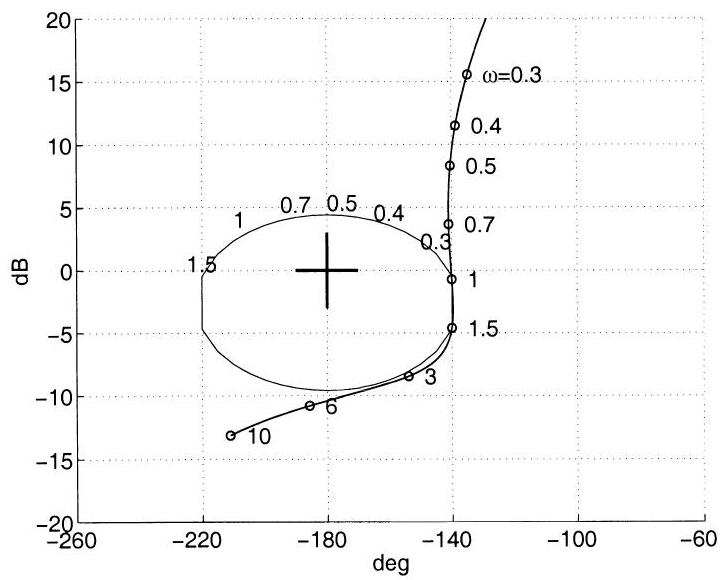
\includegraphics[max width=\textwidth]{2022_07_13_5539d24351f7cdb87589g-24}

Figura 2.17. Transmisión de bucle de $L(s)$ para la cual $\omega_{\phi}$ está cerca del máximo sujeto a $\mid 1+$ $L(j \omega) \mid>-3.5 d B$

se encuentra a partir de la siguiente aproximación de primer orden de baja frecuencia
$$
\arg \frac{1-s / z_{1}}{1+s / z_{1}} \cdots \frac{1-s / z_{n}}{1+s / z_{n}} \approx \arg \frac{1-s / z}{1+s / z}
$$
que da
$$
\frac{1}{z} \approx \frac{1}{z_{1}}+\cdots+\frac{1}{z_{n}} .
$$
Esta aproximación es válida en el rango de frecuencias donde todos los parámetros involucrados pueden ser reemplazados por la relación lineal $\tan \frac{\omega}{z_{i}} \approx \frac{\omega}{z_{i}}$. Este resultado se puede demostrar con los siguientes TF de bucle abierto que obedecen a la suposición 2.1.
$$
\begin{aligned}
&L_{1}(s)=\frac{k}{s^{2 \alpha}} \frac{3-s}{s+3}, \\
&L_{2}(s)=\frac{k}{s^{2 \alpha}} \frac{(6-s)(6-s)}{(s+6)(s+6)}, \\
&L_{d}(s)=\frac{k}{s^{2 \alpha}} e^{-s T}, T=2 / 3 .
\end{aligned}
$$
El NMP equivalente cero, $z_{0}$, de los ceros RHP de $L_{2}$ y la aproximación Pade del retardo TF, $L_{d}$, está en 3 . Estos TF se muestran en la Fig. $2.18$ con márgenes de ganancia de alrededor de $10 d B$ y márgenes de fase de aproximadamente $40^{\circ}$. Los tres TF son casi iguales incluso hasta $\omega_{M}$, el margen de ganancia de $L_{2}$ es solo $1 d B$ menos que el de $L_{1}$ y el margen de ganancia de $L_{d}$ es solo $1.5 d B$ menos. Para obtener el mismo margen de ganancia para los tres TF, la frecuencia cruzada de $L_{2}$ y $L_{d}$ debe ser de aproximadamente $0.7 \mathrm{rad} / \mathrm{sec}$, que es una desviación de menos de $12 \%$ de la de $L_{1}$.

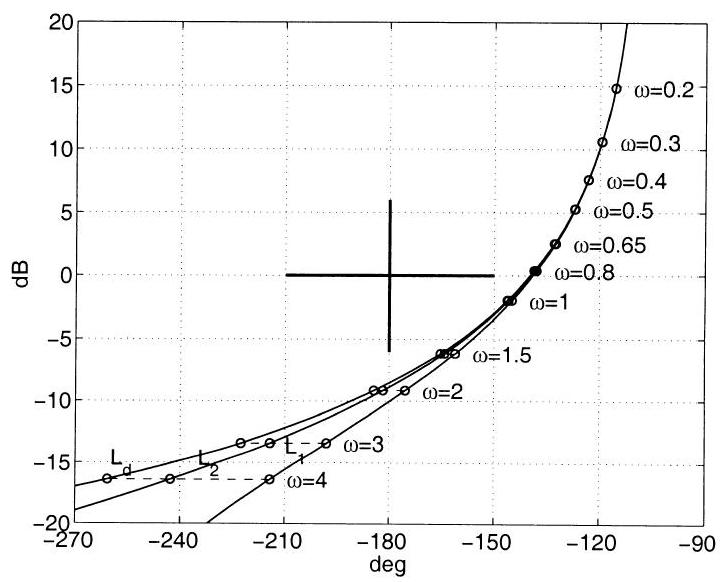
\includegraphics[max width=\textwidth]{2022_07_13_5539d24351f7cdb87589g-25}

Figura 2.18. Comparación de tres NMP TF cuya aproximación es la misma, $L_{1}$ incluye un TF de todas las pasadas con un RHP cero a $3, L_{2}$ incluye un TF de todas las pasadas con dos ceros RHP a $6, L_{d}$ incluye un retraso puro de $2 / 3$

Plantas NMP con un solo ceros RHP altamente poco amortiguados: Bajo el supuesto $2.1, L(s)$ toma una forma muy simple
$$
L(s)=\frac{k}{s^{2 \alpha}} \frac{s^{2}-2 \xi \omega s+\omega^{2}}{s^{2}+2 \xi \omega s+\omega^{2}} .
$$
Como su factor de amortiguación tiende a cero, su diagrama de Nichols converge a la estructura simple de 3 líneas rectas de la Fig. 2.19. Por lo tanto, la relación entre el margen de ganancia $M$, el margen de fase $\phi, \omega_{M}$ y la frecuencia cruzada $\omega_{\phi}$ para un complejo RHP altamente amortiguado cero en $\omega$ converge, como $\xi \rightarrow 0$, a
$$
\begin{aligned}
\phi &=\pi(1-\alpha) \\
\omega_{M} &=\omega \\
\log \frac{\omega_{\phi}}{\omega} &=\frac{M / 20}{2 \alpha} .
\end{aligned}
$$
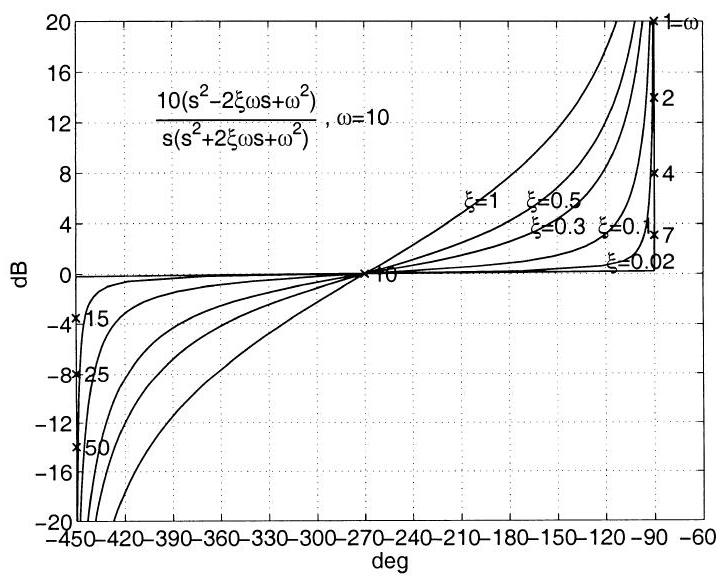
\includegraphics[max width=\textwidth]{2022_07_13_5539d24351f7cdb87589g-26}

Figura 2.19. Gráfico de Nichols de TF NMP con un solo RHP complejo cero para diferentes factores de amortiguación, $2 \alpha=1, L_{M}=1 / s$

\subsection{COMPARACIÓN CON TRANSMISIONES DE BUCLE QUE VIOLAN LA SUPOSICIÓN $2.1$}
Las relaciones entre el margen de ganancia, el margen de fase y la frecuencia cruzada como se resume en la Fig. $2.16$ ya no se mantienen si se viola la suposición $2.1$, pero siguen siendo una muy buena aproximación. Un sistema que viola la suposición $2.1$ es aquel en el que la fase mínima TF $L_{M}(s)$ tiene una ganancia mayor que la ganancia de $\frac{k}{s^{2 \alpha}}$ en el rango de frecuencia entre $\omega_{\phi}$ y $\omega_{M}$. Esto se puede expresar como una disminución en la tasa de cambio de la ganancia de bucle abierto de $L_{M}(\omega)$ con respecto a $\omega$, es decir, $\left|\frac{d L_{M}(\omega)}{d \omega}\right|$, por encima de la frecuencia de cruce $\omega_{\phi}$ en comparación con la de $k / s^{2 \alpha}$. Esto dará como resultado un aumento de $\omega_{M}$ y un aumento posterior en la ganancia del controlador requerida para frecuencias superiores a $\omega_{\phi}$. Para evaluar esta aproximación, los TF de bucle abierto NMP, con un solo RHP cero a $+1$, se formaron para satisfacer la especificación de margen $|1+L(j \omega)|>-X$ mientras intentaban aumentar la frecuencia de cruce tanto como fuera posible. La Fig. $2.20$ presenta los resultados para $X=6,3.5,2.3$ y $1.2 d B$ con márgenes de fase correspondientes de $30^{\circ}, 40^{\circ}, 50^{\circ}$, y $60^{\circ}$ respectivamente. La frecuencia de cruce en comparación con la frecuencia cruzada de la Fig. $2.16$ es $50 \%$ más para el margen de fase $30^{\circ}$, $35 \%$ más para el margen $40^{\circ}$, $10 \%$ más para el margen $50^{\circ}$ y $7 \%$ más para el margen $60^{\circ}$. Los TF de bucle abierto se formaron de tal manera que la fase en frecuencias\\

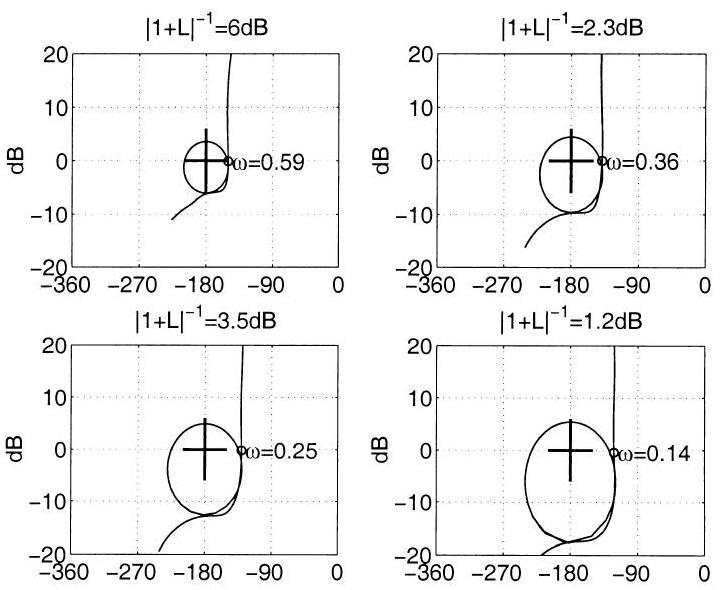
\includegraphics[max width=\textwidth]{2022_07_13_5539d24351f7cdb87589g-27}

Figura 2.20. Los bucles abiertos NMP con un solo RHP cero a $+1$ utilizados para comparar diferentes márgenes de fase, las curvas cerradas en forma ovalada son $|1+L(j \omega)|^{-1}=X d B$ donde $X=6,3.5$, $2.3$ y $1.2$ respectivamente, los bucles abiertos no deben cruzarlos

por debajo y en la frecuencia de cruce fue la misma. El aumento o la disminución de las ganancias de bucle abierto produjo diferentes frecuencias cruzadas para diferentes márgenes de ganancia. Estos resultados se resumen en la Fig. 2.21. En comparación con las frecuencias cruzadas dadas en la Fig. 2.16, un margen de fase mayor que $50^{\circ}$ da como resultado una desviación de menos de $10 \%$.

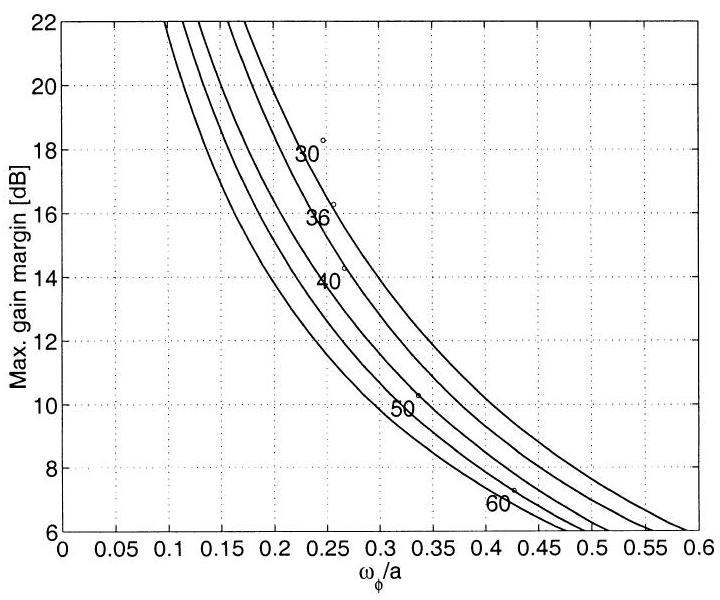
\includegraphics[max width=\textwidth]{2022_07_13_5539d24351f7cdb87589g-28}

Figura 2.21. Margen de ganancia máximo en función de un único RHP cero en $\omega_{\phi} / a$ para diferentes márgenes de fase

\subsection{PLANTAS INESTABLES}
La existencia de polos inestables coloca un límite inferior en el ancho de banda alcanzable. La gráfica de Nyquist de un bucle abierto inestable con polos RHP de $k$ debe tener cruces de $k$ del rayo $[-1,-\infty)$, por lo tanto, debe tener un margen de ganancia inferior finito, $M_{L}$. Pero un margen de ganancia superior puede no existir. Como es bien sabido, los sistemas físicos prácticos tienen al menos 2 polos más que ceros. Además, para minimizar la amplificación del ruido del sensor, las altas frecuencias deben atenuarse. Por lo tanto, el controlador debe tener más polos que ceros, y por lo tanto la fase del bucle abierto a altas frecuencias debe acercarse al menos a $-270^{\circ}$, lo que implica la existencia de $\omega_{M}$. El problema considerado aquí será: Dado un margen de ganancia más bajo $M_{L}$, margen de ganancia superior $M_{H}$, margen de fase $\phi$ y los polos RHP del sistema; Encuentra el mínimo $\omega_{\phi}$. Una representación gráfica de todos los parámetros involucrados se da en la Fig. 2.22. $0 \mathrm{~dB}$

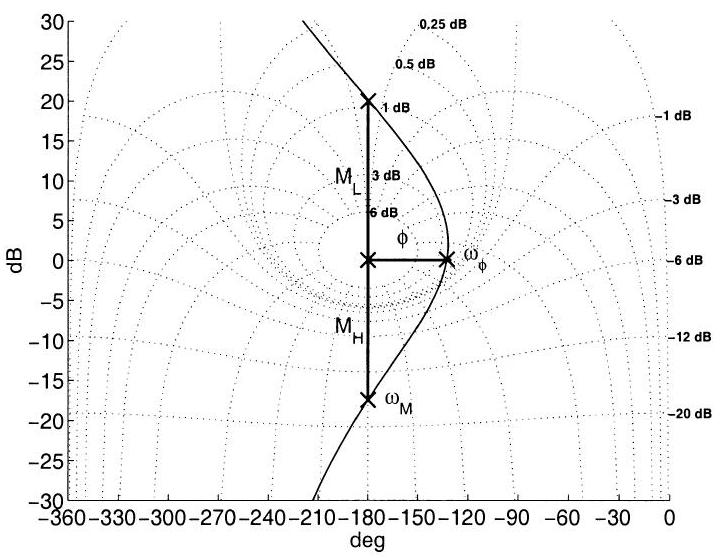
\includegraphics[max width=\textwidth]{2022_07_13_5539d24351f7cdb87589g-29}

Figura 2.22. Definición de márgenes de ganancia superior e inferior, $M_{L}, M_{H}$, margen de fase, $\phi$, frecuencia de cruce, $\omega_{\phi}$ y frecuencia de margen de ganancia, $\omega_{M}$

\subsection{PLANTAS INESTABLES CON UN SOLO POSTE RHP}
La transmisión de bucle abierto inestable más simple con un solo polo RHP y un margen de ganancia finito se utilizará para nuestra discusión, es de la forma
$$
L(s)=\frac{k}{s / a-1} \frac{\omega_{n}^{2}}{s^{2}+2 \xi \omega_{n} s+\omega_{n}^{2}} .
$$
Sin pérdida de generalidad podemos normalizar el polo tal que $a=1$ (si $a \neq 1$ las siguientes ecuaciones y resultados son verdaderos donde $\omega_{n}$ se reemplaza $a \omega_{n}, \omega_{M}$ por $a \omega_{M}$, y $\omega_{\phi}$ por $\left.a \omega_{\phi}\right)$. Usando aritmética de números complejos estándar $\left(M_{L}\right.$ en unidades aritméticas) ${ }^{3}$ :
$$
| L(j \omega)|=\frac{M_{L} \omega_{n}^{2}}{\sqrt{1+\omega^{2}} \sqrt{\left(\omega^{2}-\omega_{n}^{2}\right)^{2}+\left(2 \xi \omega_{n} \omega\right)^{2}}}
$$
${ }^{3}$ Hemos asumido que el cruce de la trama de Nyquist sobre la línea $-180^{\circ}$ tiene lugar en $\omega=0 \mathrm{rad} / \mathrm{sec}$
$$
\arg L(j \omega)=-\pi+\tan ^{-1} \omega-\tan ^{-1}\left\{\frac{2 \xi \omega_{n} \omega}{\omega_{n}^{2}-\omega^{2}}\right\}
$$
Para la frecuencia de cruce $\omega_{\phi}\left(\left| L\left(j \omega_{\phi}\right)=1\right|\right)$, la ecuación (2.9) arroja:
$$
M_{L}=\sqrt{1+\omega_{\phi}^{2}} \sqrt{\left(\omega_{\phi}^{2}-\omega_{n}^{2}\right)^{2}+\left(2 \xi \omega_{n} \omega_{\phi}\right)^{2}} / \omega_{n}^{2} .
$$
Tenga en cuenta que por consideraciones de estabilidad $M_{L}>1\left(M_{L}>0 d B\right)$, por lo tanto, la siguiente desigualdad debe mantenerse:
$$
\left(\left(\omega_{\phi}^{2}-\omega_{n}^{2}\right)^{2}+\left(2 \xi \omega_{n} \omega_{\phi}\right)^{2}\right)\left(1+\omega_{\phi}^{2}\right)>\omega_{n}^{4} .
$$
El ángulo de fase en la frecuencia superior-margen de ganancia, $\omega_{M}$, es, a partir de la ecuación (2.10), $\left(\arg L\left(j \omega_{M}\right)=-\pi\right)$ :
$$
-\pi=-\pi+\tan ^{-1} \omega_{M}-\tan ^{-1}\left\{\frac{2 \xi \omega_{n} \omega_{M}}{\omega_{n}^{2}-\omega_{M}^{2}}\right\}
$$
lo que resulta en
$$
\omega_{M}=\sqrt{\omega_{n}^{2}-2 \xi \omega_{n}}
$$
Sustituyendo la ecuación (2.13) en la ecuación (2.9) da ( $M_{H}$ en unidades aritméticas)
$$
\frac{1}{M_{H}}=\frac{\omega_{n} M_{L}}{2 \xi\left(1+\omega_{n}^{2}-2 \xi \omega_{n}\right)} .
$$
Tenga en cuenta que a partir de consideraciones de estabilidad $M_{H}<1$ in arithmetic units, hence the following inequality must hold
$$
\frac{\omega_{n} M_{L}}{2 \xi\left(1+\omega_{n}^{2}-2 \xi \omega_{n}\right)}<1 .
$$
La ecuación (2.14) y la ecuación (2.11) muestran la conexión íntima entre los márgenes de ganancia $M_{L}, M_{H}$ y la frecuencia cruzada $\omega_{\phi}$. La siguiente entidad importante es el margen de fase $\phi$. De la ecuación (2.10) satisface:
$$
\begin{aligned}
-\pi+\phi &=-\pi+\tan ^{-1} \omega_{\phi}-\tan ^{-1}\left\{\frac{2 \xi \omega_{n} \omega_{\phi}}{\omega_{n}^{2}-\omega_{\phi}^{2}}\right\} \\
\frac{2 \xi \omega_{n} \omega_{\phi}}{\omega_{n}^{2}-\omega_{\phi}^{2}} &=\frac{\omega_{\phi}-\tan \phi}{1+\omega_{\phi} \tan \phi}
\end{aligned}
$$
Mediante el uso de ecuaciones $(2.11,2.14,2.17)$ podemos obtener un conjunto de gráficos que relacionan el margen de fase $\phi$, márgenes de ganancia $M_{L}, M_{H}$ y $\omega_{\phi}$ para diferentes $\xi$ 's. Primero diferenciamos la ecuación (2.10) con respecto a $\omega$ para obtener el argumento máximo de $L(j \omega)$ en $\omega=\omega_{\phi}$. El resultado es la solución de la siguiente ecuación de 4º orden:
$$
\left(1-2 \xi \omega_{n}\right) \omega_{\phi}^{4}+\left(-2 \omega_{n}^{2}+4 \xi^{2} \omega_{n}^{2}-2 \xi \omega_{n}^{3}-2 \xi \omega_{n}\right) \omega_{\phi}^{2}+\left(\omega_{n}^{4}-2 \xi \omega_{n}^{3}\right)=0
$$
Habiendo encontrado $\omega_{\phi}$ en función de $\omega_{n}$ encontramos el margen de fase de la ecuación (2.16), y $M_{L}$ y $M_{H}$ de la ecuación (2.11) y la ecuación (2.14), respectivamente. Estas relaciones se muestran en la Fig. $2.23$ para $\xi=0.5$, donde se representa el margen de fase máximo para una frecuencia normalizada dada $\omega_{n} / a$, y el mínimo $\omega_{\phi} / a$ que se puede lograr para cada caso. Fig. $2 \cdot 24$

a)

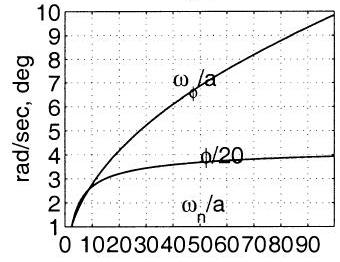
\includegraphics[max width=\textwidth]{2022_07_13_5539d24351f7cdb87589g-31}

b)

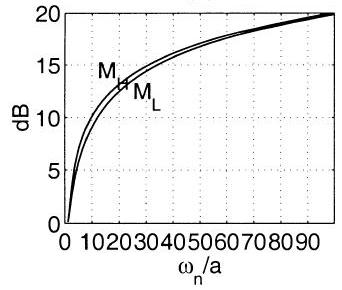
\includegraphics[max width=\textwidth]{2022_07_13_5539d24351f7cdb87589g-31(1)}

(C)

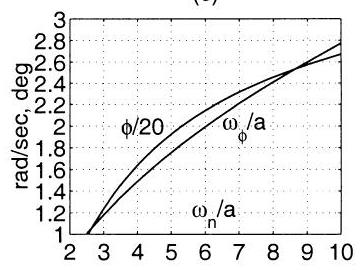
\includegraphics[max width=\textwidth]{2022_07_13_5539d24351f7cdb87589g-31(2)}

d)

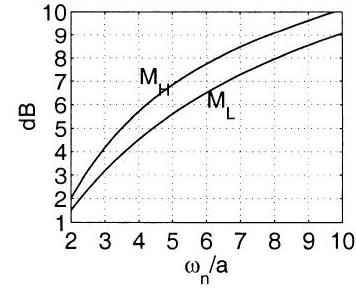
\includegraphics[max width=\textwidth]{2022_07_13_5539d24351f7cdb87589g-31(3)}

Figura 2.23. Frecuencia cruzada $\omega_{\phi}$ y margen de fase $\phi$ (superior) y márgenes de ganancia (inferior) vs. $\omega_{n}$ para $\xi=0.5$

muestra las transmisiones de bucle abierto resultantes en el gráfico de Nichols para $\omega_{n} / a=$ $3.65,5.3,8.3,14.5,33$ y 100 con márgenes de fase de $30,40,50,60,70$ y 80 grados, respectivamente. La Fig. $2.25$ es la misma que la Fig. $2.24$ pero con $\xi=1.0$. Claramente, su margen de fase es menor que para el caso $\xi=0.5$, pero su margen de ganancia es mayor.

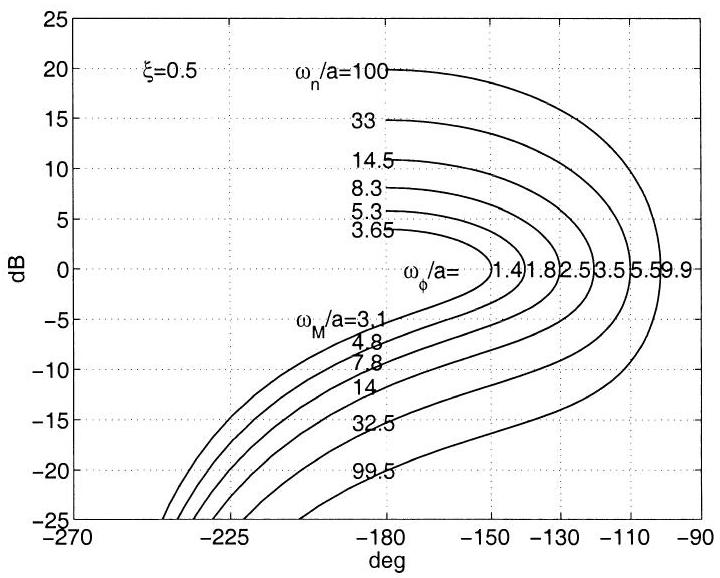
\includegraphics[max width=\textwidth]{2022_07_13_5539d24351f7cdb87589g-32}

Figura 2.24. Diagrama de ecuación de Nichols (2.8) para margen de fase máximo, $\xi=0.5$ y varios valores $\omega_{n}$

\subsubsection{UN EJEMPLO Y LIMITACIONES}
En muchos problemas prácticos de control de retroalimentación, estamos interesados en reducir $\omega_{n}$ tanto como sea posible, con el fin de minimizar la amplificación de ruido del sensor en la entrada de la planta (ver sección 3. también Horowitz (1963) y Horowitz y Sidi (1972)). Los resultados de la Fig. $2.23$ se pueden usar para encontrar las restricciones planteadas por el poste RHP de bucle abierto. Por ejemplo, supongamos que necesitamos un margen de fase de $\phi=40^{\circ}$, entonces de la Fig. $2.23 \mathrm{c}, \omega_{n} / a=5.3$ es el valor más pequeño que se puede usar, para el cual (del mismo gráfico) $\omega_{\phi} / a=1.8, M_{L}=5.8 d B$ y $M_{H}=7.2 d B$ de la Fig. 2.23d. Estos resultados son confirmados por la gráfica de Nichols de la Fig. $2.24$ en la que se muestran algunos $L(j \omega)$ 's correspondientes a la ecuación (2.8).

Las funciones prácticas de transferencia de bucle abierto tomarán formas más complicadas de lo que se supone aquí, es decir, contendrán más polos y ceros que la ecuación (2.8). Sin embargo, la configuración óptima del TF de bucle abierto (en el sentido de menor ancho de banda) tendrá las mismas características básicas de margen que se muestran para la estructura simplificada de la ecuación (2.8) y se representan en la Fig. 2.24, para las cuales los resultados de la Fig. $2.23$ se mantienen exactamente.

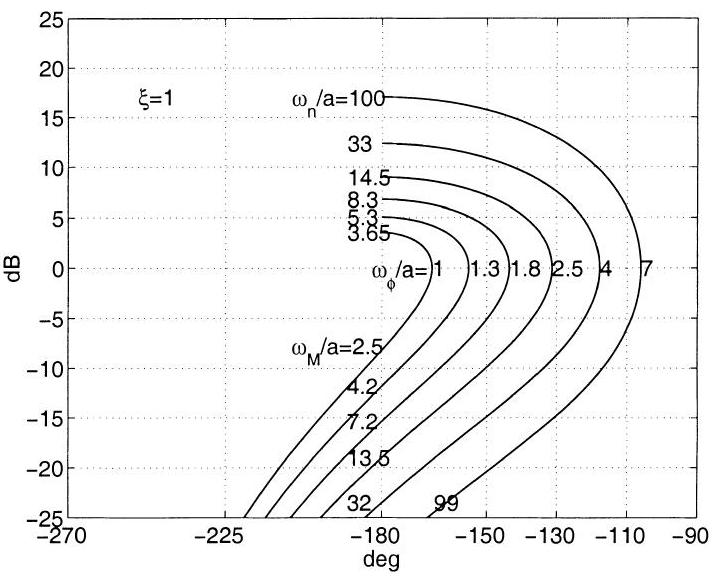
\includegraphics[max width=\textwidth]{2022_07_13_5539d24351f7cdb87589g-33}

Figura 2.25. Diagrama de Nichols de la ecuación (2.8) para el margen de fase máximo, $\xi=1$, y varios valores de $\omega_{n}$

\subsection{EXTENSIÓN A VARIOS POLOS RHP}
Plantas con solo postes RHP reales: Se puede lograr una estimación razonable de la relación entre margen de ganancia, margen de fase y frecuencia de cruce reemplazando los polos RHP por un solo polo RHP equivalente, cuya fase es la aproximación de primer orden a los polos RHP originales a altas frecuencias. Esto se debe a que la región de alta frecuencia domina las ecuaciones de ancho de banda. Una fórmula simple es: para los polos RHP ubicados en $p_{1}, \cdots, p_{n}$, el polo, $p$, que los reemplaza es la aproximación de primer orden a
$$
\arg \frac{1+p_{1} / s}{1-p_{1} / s} \cdots \frac{1+p_{n} / s}{1-p_{n} / s} \approx \arg \frac{1+p / s}{1-p / s}
$$
que da
$$
p \approx p_{1}+\cdots+p_{n} .
$$
La razón para elegir esta aproximación es que el rango de frecuencia en el que todos los parámetros involucrados es el rango donde $\omega \ll p_{i}$ y la aproximación lineal $\tan \frac{\omega}{z_{i}} \approx \frac{\omega}{z_{i}}$ es aplicable. Esta aproximación se ilustra con los siguientes TF
$$
\begin{aligned}
L_{1}(s) &=\frac{s+4}{s-4} \frac{8}{\left(s^{2} / 21.2^{2}+s / 21.2+1\right)(s+4)} \\
L_{2}(s) &=\frac{(s+1)(s+3)}{(s-1)(s-3)} \frac{8}{\left(s^{2} / 21.2^{2}+s / 21.2+1\right)(s+4)}
\end{aligned}
$$
$L_{1}$ tiene la estructura de la ecuación (2.8) con un margen de fase máximo de $40^{\circ}$ y $L_{2}$ tiene la misma estructura donde el all-pass $\frac{s+4}{s-4}$ fue reemplazado por su equivalente all-pass $\frac{(s+1)(s+3)}{(s-1)(s-3)}$. Ambas funciones de transferencia se muestran en la Fig. 2.26. Claramente, los márgenes de fase, la frecuencia cruzada y el margen de ganancia superior de $L_{2}$ están muy cerca de los de $L_{1}$, el margen de ganancia de baja frecuencia de $L_{2}$ es $1.5 d B$ menor que el de $L_{1}$, que es aproximadamente $12 \%$ de la suma de márgenes $M_{H}+M_{L}$.

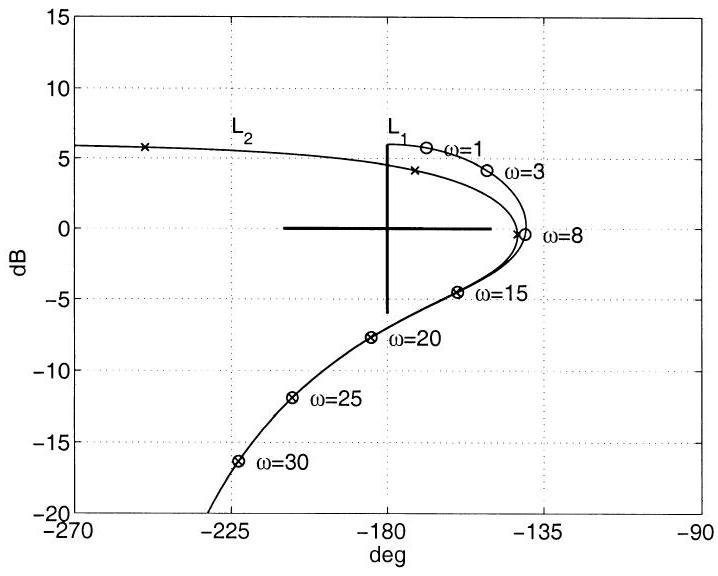
\includegraphics[max width=\textwidth]{2022_07_13_5539d24351f7cdb87589g-34}

Figura 2.26. Gráfica de Nichols de $L_{1}$ y $L_{2}$ Plantas con postes RHP muy poco amortiguados: Bajo el supuesto $2.1 L(s)$ es de la forma:
$$
L(s)=\frac{k}{s^{2 \alpha}} \frac{s^{2}+2 \xi \omega_{n} s+\omega_{n}^{2}}{s^{2}-2 \xi \omega_{n} s+\omega_{n}^{2}} .
$$
Como su factor de amortiguación, $\xi$, tiende a cero, su gráfica de Nichols converge a su forma de fase mínima en frecuencias mayores que $\omega_{n}$, y por lo tanto puede tratarse como una fase mínima $\mathrm{TF}$ en ese rango de frecuencia.

\section{FORMA DE BUCLE}
La forma de bucle es la habilidad de generar un controlador, $G(s)$, tal que un bucle abierto TF $L(s)=G P$ satisface ciertas especificaciones. Estas especificaciones pueden ser de muchos tipos, siendo la más importante que $L(s)$ satisfaga los criterios de estabilidad de Nyquist. Otros incluyen uno o más de los siguientes: margen de ganancia, margen de fase, frecuencia cruzada, ancho de banda, frecuencias de margen de ganancia, error de coeficiente (ganancia en $\omega=0$ y número de integradores en el bucle abierto) y satisfacción de los requisitos de límites. Esta sección está dedicada a ayudar al lector a dominar las habilidades de configuración de bucles a través de ejemplos.

Las dificultades en la conformación de bucles surgen debido a las relaciones de amplitud y fase dadas por la transformada de Hilbert y las integrales de Bode (Horowitz 1963), especialmente cuando la planta, $P$, es NMP y/o incluye un retardo puro y/o es inestable de bucle abierto. Esto se debe a que la estabilidad del bucle cerrado, junto con las otras especificaciones, disminuye la libertad para elegir el controlador e incluso puede imponer requisitos contradictorios, en cuyo caso no se puede crear un controlador y las especificaciones deben relajarse.

La caja de herramientas QFT Matlab ${ }^{\mathrm{TM}}$ es un paquete de software CAD utilizado por el diseñador para agregar (e iterar) TF básicos al controlador y trazar las especificaciones y la respuesta de bucle abierto en la pantalla. Estos TF básicos son:

\begin{enumerate}
  \item Ganancia simple: $k$.

  \item Polo simple o cero simple: $\frac{p}{s+p}, \frac{s+p}{p}$.

  \item Adelanto simple o retraso: $\frac{s+a}{s+b}$.

  \item Polo de segundo orden o cero: $\frac{\omega^{2}}{s^{2}+2 \xi \omega s+\omega^{2}}, \frac{s^{2}+2 \xi \omega s+\omega^{2}}{\omega^{2}}$.

  \item Mutch: $\frac{s^{2}+2 \xi_{1} \omega s+\omega^{2}}{s^{2}+2 \xi_{2} \omega s+\omega^{2}}$.

\end{enumerate}
El efecto de una ganancia simple, $k$, es desplazar $L(j \omega)$ hacia arriba en $k d B$ si $k>0 d B$ o hacia abajo si $k<0 d B$. Un polo simple ubicado en $-p$ cambia $L(j \omega)$ por $-10 \log \left(1+\omega^{2} / p^{2}\right)$ $d B$ y por $-\tan ^{-1}(\omega / p)$ deg. El cambio en $[d B, d e g]$ de un segundo orden cero y polo con diferentes factores de amortiguación, se muestra en la Fig. 2.27. El cambio en

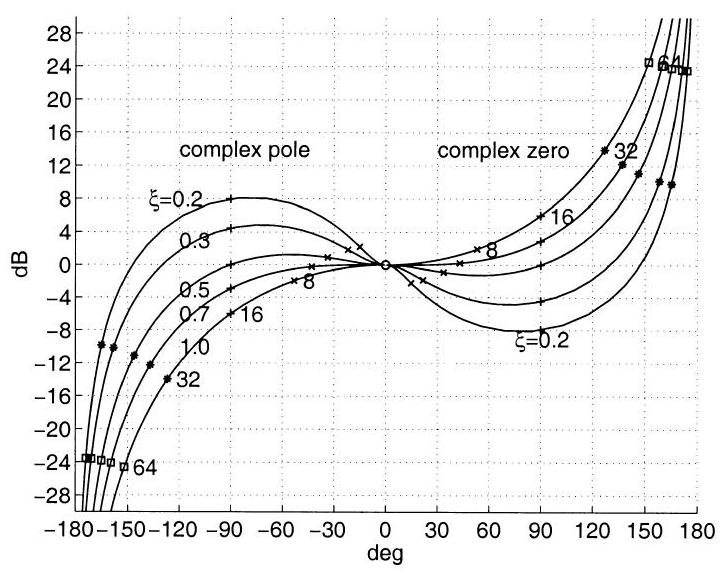
\includegraphics[max width=\textwidth]{2022_07_13_5539d24351f7cdb87589g-36}

Figura 2.27. La gráfica de Nichols del polo complejo $\left(s^{2} / 16^{2}+2 \xi / 16 s+1\right)^{-1}$ aparece en el lado izquierdo del gráfico y el cero complejo $\left(s^{2} / 16^{2}+2 \xi / 16 s+1\right)$ aparece en el lado derecho del gráfico

$[\mathrm{dB}, \mathrm{deg}]$ de un elemento lead/lag se muestra en la Fig. 2.28. Se puede demostrar, por diferenciación, que la fase máxima (mínima) de un elemento lead (lag) $\frac{s+a}{s+b}$ aparece en $\omega=\sqrt{a b}$ y es
$$
\phi=90^{\circ}-2 \tan ^{-1} \sqrt{a / b} .
$$
El cambio en $[\mathrm{dB}, \mathrm{deg}]$ de una muesca para diferentes factores de amortiguación se muestra en la Fig. 2.29.

Ejemplo 1: Dada la planta $P=10 / s$ (ver $L_{1}$ en la Fig. 2.30); se requiere dar forma a un controlador para que la transmisión de bucle general tenga una frecuencia cruzada en $\omega_{\phi}=10$, margen de fase de $45^{\circ}$ y margen de ganancia de $10 \mathrm{~dB}$.

\section{Pasos de diseño:}
\begin{enumerate}
  \item Agregue un elemento de retraso cuya fase de retraso máxima sea $45^{\circ}$ en $\omega=10$ (para lograr el margen de fase deseado en $\omega=10$ ). El elemento lag es $G_{1}=\frac{1+s / a}{1+s / b}$ donde
\end{enumerate}
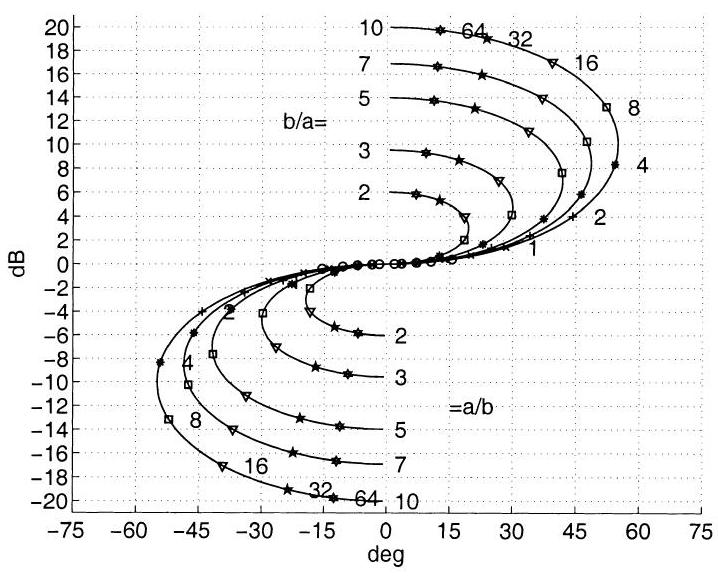
\includegraphics[max width=\textwidth]{2022_07_13_5539d24351f7cdb87589g-37}

Figura 2.28. Gráfico de Nichols del elemento principal $\frac{1+s / a}{1+s / b}$ y elemento lag $\frac{1+s / b}{1+s / a}$ para diferentes valores de $a / b$, $b=16$

$a=24, b=4$ se calculan a partir de $\sqrt{a b}=10$ y la ecuación (2.19). El TF $k_{1} G_{1} P$ se modifica por la ganancia $k_{1}=7.8 d B$ de modo que $L_{2}(j 10)=0 d B$ (mostrado en la Fig. 2.30, con la etiqueta $L_{2}$ ).

\begin{enumerate}
  \setcounter{enumi}{2}
  \item Agregue un cero tal que la fase de $L_{2}$ será aproximadamente $-90^{\circ}$ con $4 d B$ menos que el margen de ganancia deseado, es decir, $-14 d B$, (para permitir un polo complejo en el tercer paso). El elemento es $G_{2}=1+s / 45$ y el TF $k_{1} G_{1} G_{2} P$ se muestra en la Fig. $2.30$ con la etiqueta $L_{3}$.

  \item La frecuencia donde $L_{3}$ es $-4 d B$ por debajo del margen de ganancia deseado es de aproximadamente $30 \mathrm{rad} / \mathrm{sec}$. Agregar un polo complejo con un factor de amortiguación de $0.5$, cambiará $L_{3}(j 30)$ para tener una fase de $-180^{\circ}$. Se requieren iteraciones en los parámetros, incluida la ganancia para lograr los márgenes deseados. El resultado es el TF $L_{4}$ en la Fig. $2.30$ donde:

\end{enumerate}
$$
G_{4}=2.2 \frac{1+s / 24}{1+s / 4} \frac{1+s / 45}{s^{2} / 30^{2}+0.6 / 30 s+1}, \quad L_{4}=G_{4} \frac{10}{s} .
$$
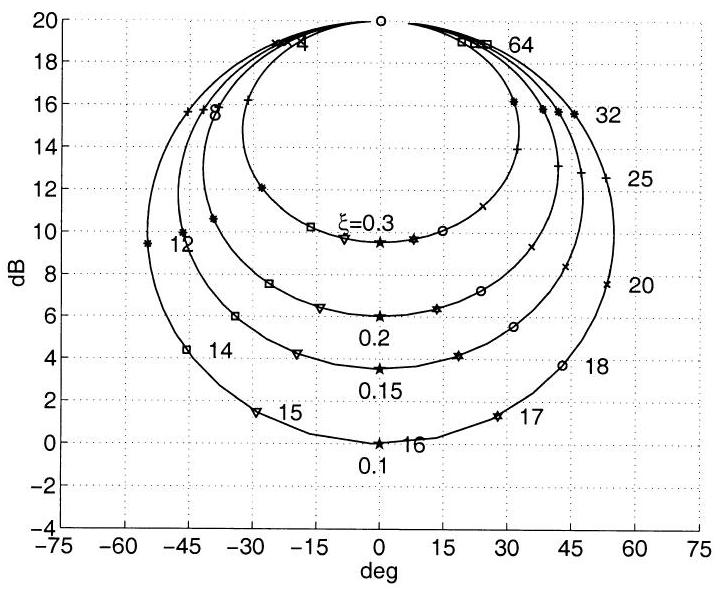
\includegraphics[max width=\textwidth]{2022_07_13_5539d24351f7cdb87589g-38}

Figura 2.29. Gráfica de Nichols del filtro Notch, $\frac{s^{2} / 16^{2}+2 \xi / 16 s+1}{s^{2} / 16^{2}+2 / 16 s+1}$, para diferentes factores de amortiguación, $\xi$

Ejemplo 2: Dada la planta $P=10 / s^{2}$; se requiere dar forma a un controlador para que la transmisión de bucle general tenga una frecuencia cruzada $\omega_{\phi}=10$, margen de fase de $45^{\circ}$ y margen de ganancia de $10 d B$.

\section{Pasos de diseño:}
\begin{enumerate}
  \item Agregue un elemento principal cuya fase de avance máxima sea $45^{\circ}$ en $\omega=10$ (para lograr el margen de fase deseado en $\omega=10)$. El elemento es $G_{1}=$ $(1+s / a) /(1+s / b)$ donde $a=4, b=24$ se calculan a partir de $\sqrt{a b}=10$ y ecuación (2.19). El TF $k_{1} G_{1} P$ se modifica por la ganancia $k_{1}=12.3 d B$ y el resultado $L_{2}(j 10)=0 d B$ se muestra en la Fig. 2.31.

  \item Agregue un cero tal que la fase de $L_{2}$ será aproximadamente $-110^{\circ}$ con $4 d B$ menos que el margen de ganancia deseado, es decir, $-14 d B$, (para permitir un polo complejo en el tercer paso). El elemento es $G_{2}=1+s / 50$ y el TF $k_{1} G_{1} G_{2} P$ se muestra en la Fig. $2.31$ etiquetada como $L_{3}$.

  \item La frecuencia donde $L_{3}$ es $-4 d B$ por debajo del margen de ganancia deseado es de aproximadamente $30 \mathrm{rad} / \mathrm{sec}$. Agregar un poste complejo con un factor de amortiguación de $ 0.5 $,

\end{enumerate}
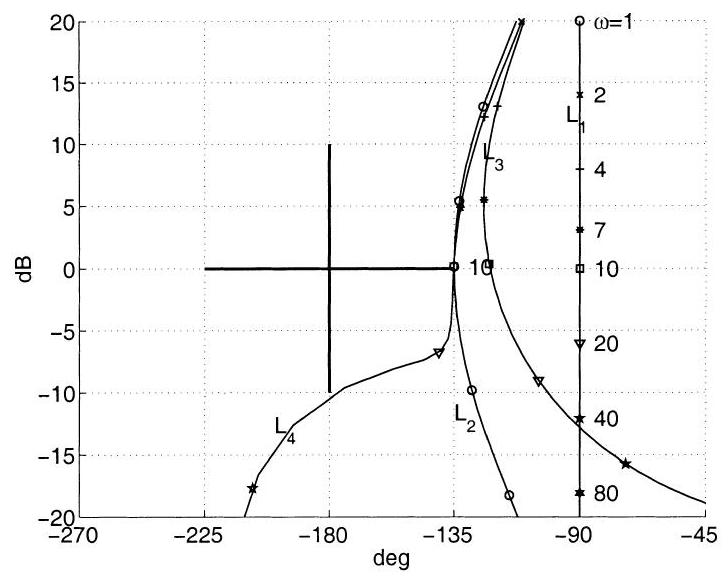
\includegraphics[max width=\textwidth]{2022_07_13_5539d24351f7cdb87589g-39}

Figura 2.30. Gráfica de Nichols para $10 d B$ de margen de ganancia y $45^{\circ}$ de margen de fase, la planta es de $10 / \mathrm{s}$

Cambie $L_{3}(j 30)$ para tener una fase de $-180^{\circ}$. Se requieren iteraciones en los parámetros, incluida la ganancia para lograr los márgenes deseados. El resultado es el TF $L_{4}$ en la Fig. $2.31$
$$
G_{4}=[12.3 d B] \frac{1+s / 4}{1+s / 24} \frac{1+s / 50}{s^{2} / 40^{2}+0.8 / 40 s+1}, \quad L_{4}=G_{4} \frac{10}{s^{2}} .
$$
Ejemplo 3: La Fig. $2.32$ describe un conjunto de límites, para la planta nominal $P=$ $\frac{k}{s(s+10)}$. Se requiere dar forma a $G(s)$, de tal manera que $L(j \omega)=P G(j \omega)$ estará por encima de las curvas marcadas $B(2), B(4), B(8)$ y $B(20)$ a $\omega=2,4,8,20$, respectivamente, y fuera de la curva cerrada en todas las frecuencias. El primer paso es ajustar la ganancia nominal de la planta para satisfacer los límites de baja frecuencia, marcados como ' $a$ ' en la Fig. 2.32. Los límites se cumplen excepto alrededor de $\omega=80$, por lo tanto el segundo paso es añadir un elemento principal cuya derivación máxima sea alrededor de $\omega=80$, ver bucle marcado ' $b$ '. Aunque los límites se satisfacen con el bucle 'b', queremos agregar otro polo al controlador para lograr buenas características de roll-off a altas frecuencias, y esto se hace de la siguiente manera: Agregue un cero de modo que aproximadamente $ 4 d B$ por debajo de la parte inferior de los límites a frecuencias altas, $ -28 d B$, la fase de

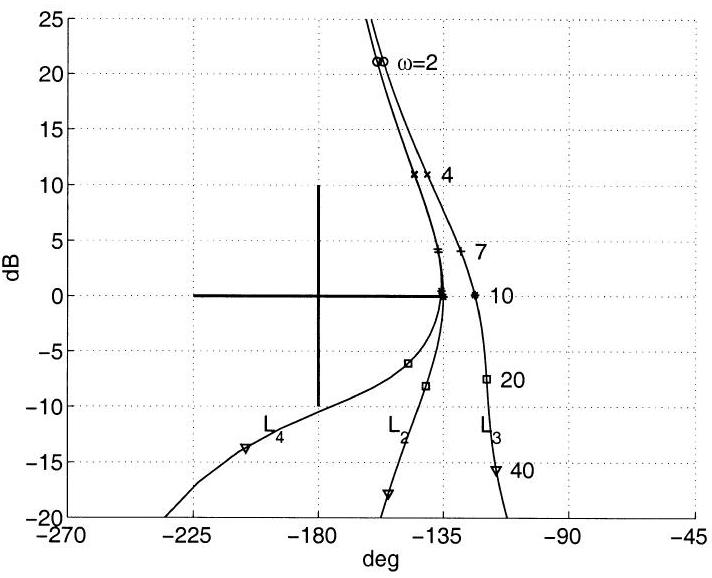
\includegraphics[max width=\textwidth]{2022_07_13_5539d24351f7cdb87589g-40}

Figura 2.31. Gráfica de Nichols para $10 d B$ de margen de ganancia y $45^{\circ}$ de margen de fase, la planta es de $10 / \mathrm{s}$

La transmisión de bucle es alrededor de $-120^{\circ}$, ver curva ' $\mathrm{c}$ '; Luego agregue un polo complejo con amortiguación $\xi = 0.5$ y frecuencia natural que tocará los límites, vea Transmisión de bucle 'D'.

El proceso de diseño descrito en el ejemplo 3 es adecuado para un gran conjunto de ejemplos prácticos y procede de la siguiente manera:

\begin{enumerate}
  \item Comience con una ganancia simple para satisfacer las especificaciones de baja frecuencia (conocidas en QFT como límites).

  \item Agregue elementos de derivación y/o retraso para satisfacer los límites de baja frecuencia y al mismo tiempo disminuir la amplificación del controlador.

  \item Agregue elementos principales para satisfacer los límites de alta frecuencia.

  \item Iterar en los parámetros del controlador para disminuir el ancho de banda del controlador intentando disminuir su ganancia de alta frecuencia.

  \item Agregue tantos polos de exceso sobre ceros como sea necesario, agregando un cero (s) y luego un polo (s) lo suficientemente lejos o un par de polos complejos.

\end{enumerate}
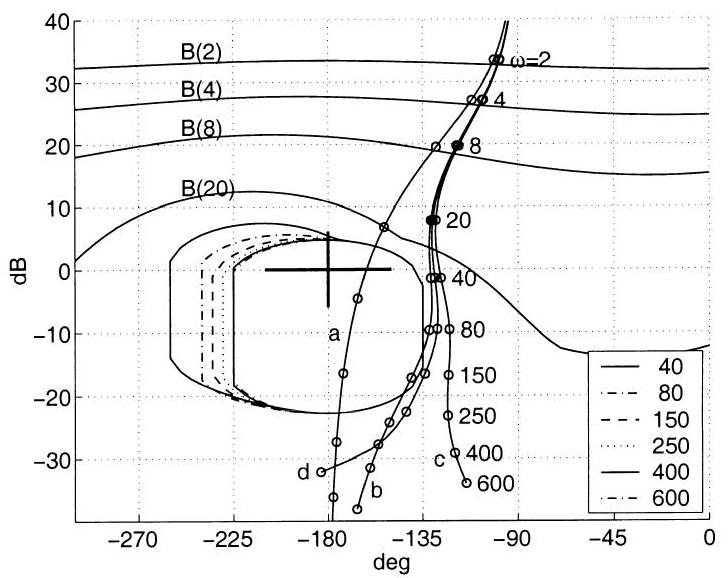
\includegraphics[max width=\textwidth]{2022_07_13_5539d24351f7cdb87589g-41}

Figura 2.32. Pasos de conformación de bucles a, b, c y diseño final d, por ejemplo 3

El paso final puede implicar iteraciones en los parámetros de control o la adición de muchos elementos de plomo y retraso seguidos de un procedimiento de reducción del modelo: la caja de herramientas QFT Matlab ${ }^{\mathrm{TM}}$ (Borghesani et al. 1994) es muy adecuado para este proceso. Finalmente es recomendable hacer los ejercicios al final de este capítulo. No tenemos ninguna duda de que usando la caja de herramientas QFT de Matlab ${ }^{\mathrm{TM}}$, uno puede obtener una buena habilidad en la configuración de bucles en un día más o menos.

\section{RESÚMEN}
En este capítulo revisamos los parámetros clásicos básicos que caracterizan un sistema de retroalimentación: márgenes, ancho de banda y frecuencia cruzada. Se enfatizó que estos parámetros pueden servir como excelentes figuras de mérito para la robustez y el desempeño de un sistema de retroalimentación. Sin embargo, la existencia de varias frecuencias cruzadas invalida lo que se dijo anteriormente.

Un controlador está diseñado para cumplir con las especificaciones de bucle cerrado deseadas, y se definen las especificaciones de dominio de tiempo y dominio de frecuencia. Aunque no existe una traducción uno a uno del dominio del tiempo a las especificaciones del dominio de la frecuencia, se proponen dos algoritmos que intentan cerrar la brecha. i)

\section{Capítulo 3}
\section{SÍNTESIS DE CONTROLADORES LTI PARA PLANTAS MISO LTI}
\section{INTRODUCCIÓN}
En este capítulo se presenta la herramienta de ingeniería para el diseño de retroalimentación de sistemas de salida única y salida única de entrada múltiple, conocida como QFT. Las características importantes de este enfoque son: $(i)$ es robusto a la cantidad exacta de incertidumbre de la planta; ii) adapta el circuito cerrado con precisión a las especificaciones que se dan en cada frecuencia; y (iii) la técnica se basa gráficamente, lo que permite comprender las compensaciones entre los parámetros de diseño, como la complejidad, la programación, la cantidad de incertidumbre, el tiempo de muestreo, los márgenes y el ancho de banda. Como resultado, el método permite al diseñador crear diseños de bajo ancho de banda.

El método de diseño se desarrolla por separado para uno y dos sistemas de grado de libertad, y se dan los algoritmos para calcular límites. Luego se extiende a los sistemas de datos muestreados y plantas de NMP, y se proporciona una explicación detallada del fenómeno NMP.

\section{UN SISTEMA DOF}
El sistema de retroalimentación de interés se representa esquemáticamente en la Fig. $3.1$ y se describe mediante las ecuaciones:
$$
\begin{aligned}
y &=P u+P_{d} d \\
u &=-G H y+G n .
\end{aligned}
$$
El problema discutido en la secuela es cómo diseñar un controlador, $G(s)$, tal que para un conjunto dado de plantas, $\{P\}$, el bucle cerrado es estable y se cumplen ciertas especificaciones de dominio $\omega$. Todas las especificaciones de $\omega$-domain para un DOF

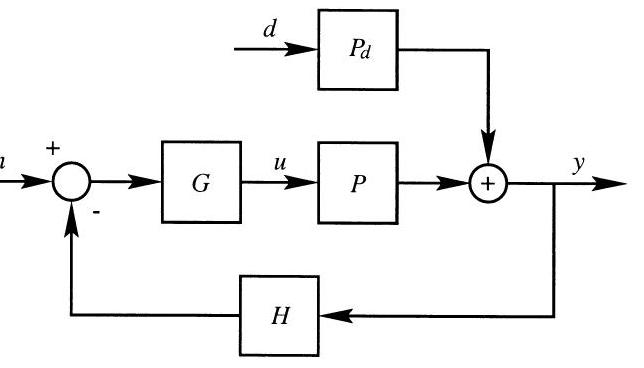
\includegraphics[max width=\textwidth]{2022_07_13_5539d24351f7cdb87589g-43}

Figura 3.1. Un único sistema de retroalimentación único DOF

Los sistemas se pueden reducir a la siguiente desigualdad en el controlador $G(s)$ :
$$
\left|\frac{A(j \omega)+B(j \omega) G(j \omega)}{1+P H G(j \omega)}\right| \leq \delta(\omega), \forall P \in\{P\},
$$
donde $A, B, C$ y $\delta$ pueden depender de la planta $P$, así como de $\omega$. Todas las especificaciones del dominio $\omega$, $\delta(\omega)$, son valores absolutos y, por lo tanto, solo funciones de $\omega$ (es decir, la fase no es importante en lo que respecta a las especificaciones). Distinguimos entre las siguientes dos categorías principales de problemas:

\begin{enumerate}
  \item Reducción de sensibilidad: las especificaciones son:
\end{enumerate}
$$
\left|\frac{1}{1+P H G(j \omega)}\right| \leq \delta_{s}(\omega) .
$$
Tenga en cuenta que $G(j \omega)=\infty$ es siempre una solución.

\begin{enumerate}
  \setcounter{enumi}{2}
  \item Minimización del esfuerzo de control: las especificaciones adoptan la forma:
\end{enumerate}
$$
\left|\frac{G(j \omega)}{1+P H G(j \omega)}\right| \leq \delta_{c}(\omega)
$$
Tenga en cuenta que $G(j \omega)=0$ es siempre una solución a la desigualdad anterior.

El problema de reducción de sensibilidad tiende a aumentar la ganancia del bucle, mientras que el problema del esfuerzo de control pone un límite superior en la salida del controlador (suponiendo $\left.\delta_{c}<|P H|^{-1}\right)$. Todas las especificaciones de dominio $\omega$-domain de la sección $3.2$ para el problema DOF se pueden reducir a una de las dos categorías anteriores. A continuación se presentan dos ejemplos. Ejemplo 1: Para un $d(s)$ y $P_{d}(s)$ dados, requerimos que la producción de la planta $y$ de la Fig. 3.1, esté limitada por $e(\omega)$. Este problema se puede reformular en forma de un problema de reducción de sensibilidad de la siguiente manera:
$$
\left|\frac{1}{1+P H G(j \omega)}\right| \leq \frac{e(\omega)}{\left| P_{d} d(j \omega)\right|} \equiv \delta_{s}(\omega)
$$
Ejemplo 2: Para un determinado $n(s)$ en la Fig. 3.1, requerimos que la entrada de la planta esté limitada por $e(\omega)$. Esto puede escribirse como un problema de esfuerzo de control:
$$
\left|\frac{G(j \omega)}{1+P H G(j \omega)}\right| \leq \frac{e(\omega)}{|n(j \omega)|} \equiv \delta_{u}(\omega)
$$

\subsection{PROBLEMA DE REDUCCIÓN DE SENSIBILIDAD}
Considere el sistema que se muestra en la Fig. 3.1, donde $P$ es una planta LTI. El problema al que nos enfrentamos es cómo diseñar un controlador, $G(s)$, tal que, para un conjunto dado de plantas, $\{P\}$, el bucle cerrado sea estable y la sensibilidad del bucle abierto satisfaga las especificaciones de la forma:
$$
\left|\frac{1}{1+G P H(j \omega)}\right| \leq \delta_{s}(\omega), \forall P \in\{P\} .
$$
Tenga en cuenta que $\delta_{s}(\omega)$ y $H(j \omega)$ pueden depender de la planta, $P$. La solución a la desigualdad (3.1), para una frecuencia dada $\omega$, planta $P(j \omega)$, y sensor TF $H(j \omega)$, es un círculo en el plano complejo. Usando la notación $L(s)=P G H$, entonces el exterior del círculo centrado en $[-1,0]$ con radio $\left|\delta_{s}(\omega)\right|^{-1}$ es la región permitida para la cual la desigualdad (3.1) es válida para $L(j \omega)$ (ver Fig. 3.2), mientras que el área interior no lo es. Del mismo modo, $G(j \omega)$ define otro círculo en el plano complejo, fuera del cual se satisfará la desigualdad (3.1) (ver Fig. 3.2). El proceso de diseño será:

\begin{enumerate}
  \item Calcula círculos en cada frecuencia para todas las plantas $P \in\{P\}$, denotando la curva de la unión de todos los círculos en un $\omega$ dado por $B(\omega)$. En el lenguaje QFT, $B(\omega)$ es el límite de $G(s)$ a la frecuencia $\omega$.

  \item Encuentra (forma) un TF $G(s)$ tal que a cualquier frecuencia $\omega, G(j \omega)$ se encuentra fuera del límite $B(\omega)$, de conformidad con la desigualdad (3.1), y el bucle cerrado es estable para todos los $P \in\{P\}$

\end{enumerate}
El $G(s)$ resultante será entonces una solución, en la medida en que el circuito cerrado sea estable y satisfaga las especificaciones. A partir de la geometría simple, se puede demostrar que el centro del círculo prohibido, para el parámetro $L(j \omega)=G P H(j \omega)$, se encuentra en $[-1,0]$ y su radio es $\delta_{s}^{-1}(\omega)$. Para el parámetro $G(j \omega)$ el centro se desplaza a $-1 / P H(j \omega)$ y el radio es, en consecuencia, $\delta_{s}^{-1} /| P H(j \omega)|$. Sin embargo, no se recomienda el cálculo de estos límites con la ayuda de los círculos correspondientes. El procedimiento preferido (también el utilizado por QFT Matlab ${ }^{\mathrm{TM}}$ toolbox, Borghesani et al. (1994)) se presentará a continuación.

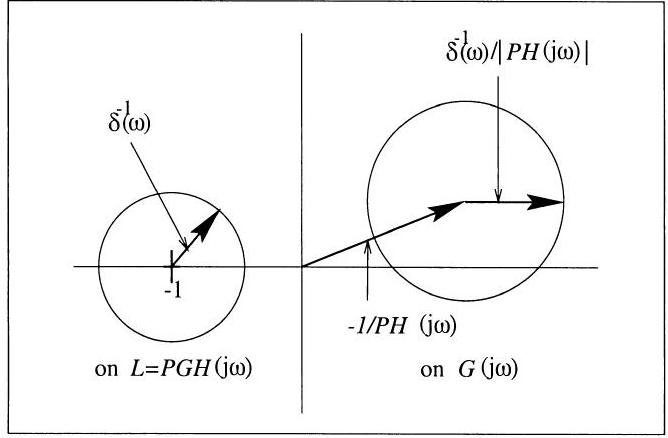
\includegraphics[max width=\textwidth]{2022_07_13_5539d24351f7cdb87589g-45}

Figura 3.2. El círculo de la izquierda con un radio de $\delta_{s}^{-1}(\omega)$ y centrado en $[-1,0]$ define la región permitida para $L(j \omega)=G P H(j \omega)$. El círculo de la derecha con radio $\frac{\delta_{0}^{-1}}{| P H(j \omega)|} $ centrado en $-1 / P H(j \omega)$ define la región permitida para $G(j \omega)$

\subsection{CÁLCULOS ENLAZADOS}
Con la forma polar de $G(j \omega)$, a una frecuencia dada, $\omega$, es decir, $G(j \omega)=g e^{j \phi}$ y $P H(j \omega)=p e^{j \theta}$, la desigualdad (3.1) se reduce a:
$$
\left|\frac{1}{1+g p e^{j(\phi+\theta)}}\right| \leq \delta(\omega) .
$$
Las magnitudes cuadradas de ambos lados de la desigualdad se convierten en:
$$
\frac{1}{g^{2} p^{2}+2 g p \cos (\phi+\theta)+1} \leq \delta^{2}(\omega) .
$$
Reorganizar los términos nos da la forma cuadrática:
$$
G^{2} p^{2}+2 g p \cos (\phi+\theta)+1-1 / \delta^{2}(\omega) \geq 0 .
$$
El parámetro desconocido en la ecuación anterior es el número complejo $g e^{j \phi}$, que es un círculo para todo $\phi \in[0,2 \pi]$, (véase también Thompson (1995)). La curva de la unión de todos estos círculos es el límite $B(\omega)$. En la práctica, no es posible calcular estos límites para todos los $\omega$ y un número infinito de plantas, por lo tanto, el algoritmo de cálculo de límite propuesto es:

\begin{enumerate}
  \item Discretiza las frecuencias $[0, \infty)$ en un conjunto finito $\Omega=\left\{\omega_{1}, \cdots, \omega_{m}\right\}$.

  \item Discretiza el conjunto de plantas inciertas en un conjunto finito $\{P\}=\left\{P_{1}, \cdots, P_{n}\right\}$.

  \item Discretiza la fase del controlador $\phi$ en un conjunto ordenado, por ejemplo $\Phi=\{0,-5, \cdots,-360\}$

  \item Elija una sola frecuencia $\omega \in \Omega$.

  \item Elija una sola fase $\phi \in \Phi$.

  \item Elija una sola planta $P_{i}$ desde $\{P\}$.

  \item Compute $g_{\max }\left(P_{i}(j \omega), \phi\right)$ and $g_{\min }\left(P_{i}(j \omega), \phi\right)$ using inequality (3.2).

  \item Repita el paso 7 para todos los $P_{i}(j \omega)$ y denote

\end{enumerate}
$$
\begin{aligned}
g_{\max }(\phi, \omega) &=\max _{P_{i}} g_{\max }\left(P_{i},(j \omega), \phi\right) \\
g_{\min }(\phi, \omega) &=\min _{P_{i}} g_{\min }\left(P_{i},(j \omega), \phi\right) .
\end{aligned}
$$

\begin{enumerate}
  \setcounter{enumi}{9}
  \item Repita los pasos $5-8$ para todas las fases de $\Phi$.

  \item Repita los pasos $4-9$ para todas las frecuencias en $\Omega$.

\end{enumerate}
Para un $\omega \in \Omega$ y fase $\phi \in \Phi$, el intervalo a partir del cual $| G(j \omega)|$ se permite tomar sus valores es:
$$
\begin{aligned}
| G(j \omega)| \leq g_{\min } \text { o }| G(j \omega)| & \geq g_{\max }, \text { if } g_{\min }(\phi, \omega)>0 \\
| G(j \omega)| & \geq g_{\max }, \text { if } g_{\min }(\phi, \omega) \leq 0,
\end{aligned}
$$
y su curva (sobre todo $\phi \in \Phi)$ es el límite $B(\omega)$ en $G(j \omega)$. Establecer los límites en $L_{0}=G P_{0} H$ para una planta en particular $P_{0}$, desde $\{P\}$, en lugar de en $G$, es más natural para la conformación de bucles; los límites en $L_{0}(j \omega)$ son los mismos que en $G(j \omega)$ pero cada punto delimitador, digamos $z$, se desplaza a $z / P_{0} H(j \omega)$.

Ejemplo: Dado el $k de la planta / s$ donde $k \in[1,3]$, se requiere que la producción de la planta sea inferior a $\omega / 5$, pero no superior a $1.4$, es decir, $\delta=\min (\omega / 5,1.4)$. Los conjuntos discretos para (pasos $1,2,4)$ son: $\Omega=\{1,2,4,8\} ; \phi=\{0,-5, \cdots,-360\}$; y $\{P\}=\{1 / s, 2 / s, 3 / s\}$. Los límites de $G$ se calculan mediante el algoritmo descrito en los pasos $4-10$. La desigualdad a resolver es
$$
\left|\frac{1}{1+P G(j \omega)}\right| \leq \min \left(\frac{\omega}{5}, 1.4\right)=\delta(\omega)
$$
que para una frecuencia dada, $\omega$, valor de planta $p e^{j \theta}$ y fase controladora, $\phi$, reduce a la siguiente desigualdad en la amplitud del controlador $g$
$$
G^{2} p^{2}+2 g p \cos (\phi+\theta)+1-1 / \delta^{2}(\omega) \geq 0 .
$$
Los límites de $L_{0}=G P_{0}$ para $P_{0}=1 / s$ se muestran en la Fig. $3.3$

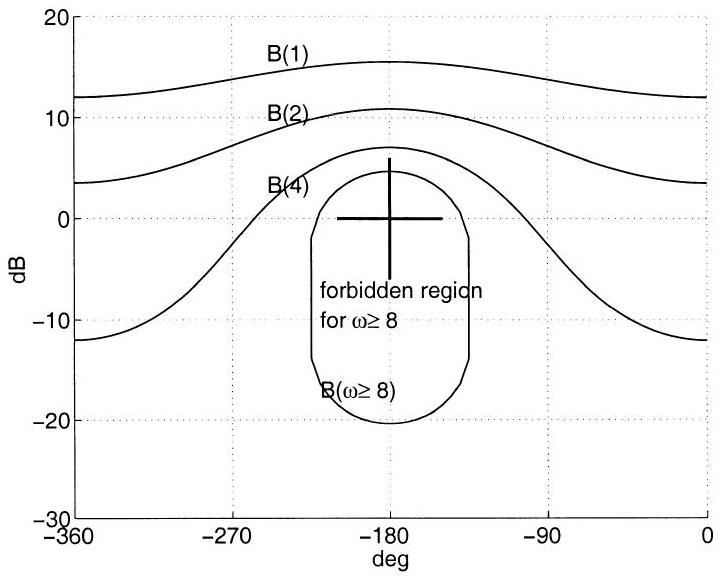
\includegraphics[max width=\textwidth]{2022_07_13_5539d24351f7cdb87589g-47}

Figura 3.3. La región por encima de las curvas delimitadoras $B(\omega), \omega=1,2,4$, son las regiones permitidas para la ubicación de $L_{0}(j \omega)$, mientras que para $\omega \geq 8$, la región fuera de la curva cerrada define el conjunto de ubicaciones permitidas para $L_{0}(j \omega)$

\subsection{PROBLEMA DE ESFUERZO DE CONTROL}
Considere el sistema que se muestra en la Fig. 3.1, donde $P$ es una planta LTI. Nuestro problema es cómo diseñar un controlador, $G(s)$, tal que para un conjunto dado de plantas, $\{P\}$, el bucle cerrado es estable y satisface las especificaciones de la forma:
$$
\left|\frac{G(j \omega)}{1+G P H(j \omega)}\right| \leq \delta_{u}(\omega), \forall P \in\{P\} .
$$
Tenga en cuenta que $\delta_{u}(\omega)$ y el sensor TF, $H(s)$, pueden depender de la planta, $P$. La solución a la desigualdad (3.3) en cada frecuencia para una planta dada, puede ser descrita por un círculo en el plano complejo. Para determinar si el interior del círculo es parte de la región permitida, basta con verificar qué sucede cuando $G(j \omega) \equiv \infty$. Si $G(j \omega) \equiv \infty$, está en la región permitida, entonces $\delta_{u}| P H(j \omega)|>1$, es decir, la región exterior a este círculo se ajusta a la desigualdad (3.3) mientras que el área interior no. Sin embargo, si $\delta_{u}| P H(j \omega)|<1$, inequality (3.3) is true within the above circle's interior. El proceso de diseño será:

\begin{enumerate}
  \item Calcula los círculos correspondientes a la desigualdad (3.3) en cada frecuencia y para todos los $P \in\{P\}$. Intersecar todas las regiones permitidas de todos los círculos calculados para un $\omega$, denotando la curva resultante por $B(\omega)$.

  \item Encuentra (forma) un TF, $G(s)$, tal que a cualquier frecuencia $\omega, G(j \omega)$ se encuentra dentro de su límite $B(\omega)$ de conformidad con la desigualdad (3.3) y el bucle cerrado es estable para todos los $P \in\{P\}$.

\end{enumerate}
$G(s)$ se dirá entonces que es una solución al problema del esfuerzo de control.

A partir de consideraciones geométricas simples, se puede demostrar que el centro del círculo que resuelve la desigualdad:
$$
\left|\frac{L}{1+L}\right|<a
$$
se encuentra en $\left[a^{2} /\left(1-a^{2}, 0\right]\right.$ y su radio es $a / \left|1-a^{2}\right|$. Además, si $a<$ $1(a="">1)$ su interior (exterior) es la región permitida. Por lo tanto, la solución a la desigualdad (3.3) para $P H G$ es el mismo círculo con $a=\delta /| P H|$; y para el parámetro $G$, ya que $G=\frac{L}{P H}$, es el círculo cuyo centro, denotado por $C_{g}$, y radio, denotado por $R_{g}$, son
$$
C_{g}(\omega)=\frac{a^{2}}{\left(1-a^{2}\right) P H(j \omega)}, R_{g}(\omega)=\frac{a}{\left|1-a^{2}\right|| P H(j \omega)|} .
$$
Sin embargo, no se recomienda el cálculo de estos límites con la ayuda de los círculos correspondientes. El procedimiento preferido se presentó en la sección $2.2$.

Ejemplo: Para la planta $1 / s$, se requiere que la entrada de planta de circuito cerrado a $\omega=1$ sea inferior a $1.1$ y menor que $0.14$ (unidades aritméticas) a $\omega=5$. Las curvas (límites) en $L_{0}(j \omega)=G P_{0}(j \omega)$ para $P_{0}=1 / s$ se muestran en la Fig. 3.4. Para $\omega=1$, es el interior de la curva cerrada la región prohibida, mientras que para $\omega=5$ el área por debajo de la curva abierta es la región permitida.

\subsection{EJEMPLOS}
Ejemplo 1: Dada una planta incierta que incluye un integrador, un polo simple a $-1$, y una ganancia incierta en el intervalo $[1,5]$
$$
\{P\}=\frac{k}{s(s+1)}, k \in[1,5],
$$
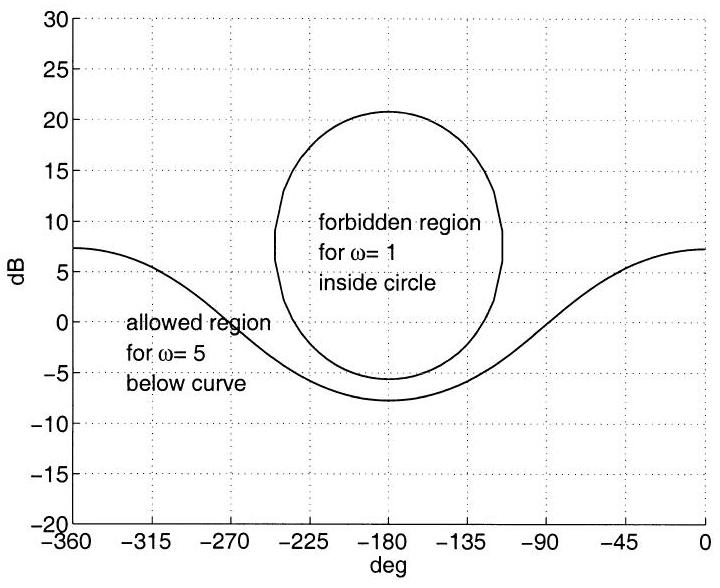
\includegraphics[max width=\textwidth]{2022_07_13_5539d24351f7cdb87589g-49}

Figura 3.4. Límites en el esfuerzo de control: para $\omega=1$ el interior de la curva cerrada es la región prohibida para $L_{0}(j \omega)$, mientras que para $\omega=5$ el área por debajo de la curva abierta es la región permitida para $L_{0}(j \omega)$. En el plano complejo, con escalas aritméticas reales e imaginarias, ¡ambas curvas son círculos!

el requisito es diseñar un controlador tal que para cualquier planta en $\{P\}$ : i) el circuito cerrado es estable, (ii) a frecuencias $[1,2,4] \mathrm{rad} / \mathrm{sec}$, la sensibilidad es inferior a $[0.05,0.2,0.8]$ unidades aritméticas, respectivamente; y (iii) en todas las frecuencias, márgenes de ganancia y fase de la forma $|1+L(j \omega)|^{-1}<3.5 d B$ are satisfied.

Los límites y los dos diseños se muestran en la Fig. $3.5$ y la Fig. $3.6$ donde la planta nominal es $1 /\left(s^{2}+s\right)$. El controlador diseñado en la Fig. $3.5$ es
$$
G_{1}=28 \frac{(1+s / 30)(1+s / 6)}{(1+s / 20)(1+s / 90)(1+s / 220)},
$$
y se compone solo de polos y ceros reales, mientras que el segundo diseño del controlador, que aparece en la Fig. 3.6, y es
$$
G_{2}=28 \frac{(1+s / 27)(1+s / 6)}{(1+s / 14)} \frac{78^{2}}{s^{2}+78 s+78^{2}},
$$
consiste en un par de polos complejo con una relación de amortiguación de $ 0.5 $. El segundo diseño es mejor en el sentido de que el ruido del sensor de alta frecuencia en la entrada de la planta se reduce, en comparación con el primer diseño. Una comparación, en forma de un diagrama de Bode de los dos TF desde la salida del sensor hasta la entrada de la planta, se representa en la Fig. 3.7. Tenga en cuenta que el algoritmo de conformación de bucles intenta posicionar la respuesta de bucle abierto en cada frecuencia, lo más cerca posible de su curva límite correspondiente, en la región permitida, lo que naturalmente impone una solución de ancho de banda más pequeña (Horowitz (1978) apéndice 1). Dado que a altas frecuencias el

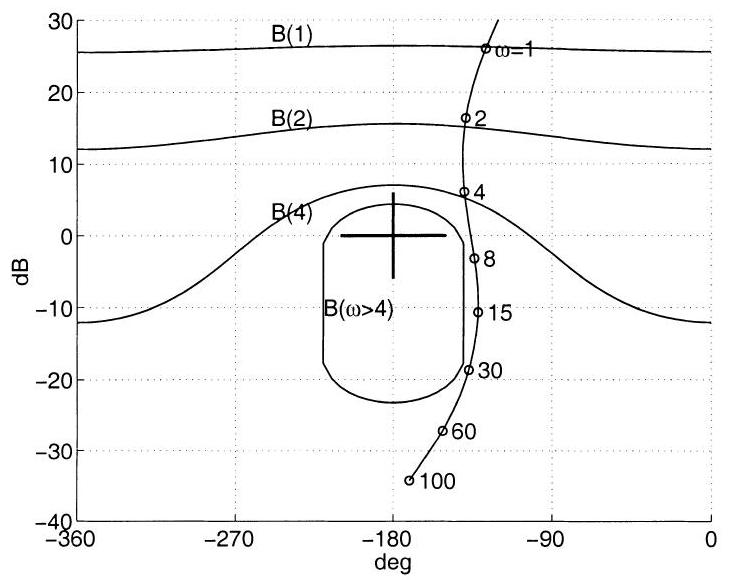
\includegraphics[max width=\textwidth]{2022_07_13_5539d24351f7cdb87589g-50}

Figura 3.5. Límites y $L_{1}=G_{1} P_{0}$

Los beneficios de la retroalimentación son insignificantes, cualquier especificación a altas frecuencias dará como resultado un gran ancho de banda con una mejora insignificante del rendimiento del bucle cerrado. A partir de los límites en $\omega=4$ podemos esperar que a frecuencias más altas, la ganancia de bucle abierto será inferior a $0 d B$, y por lo tanto las especificaciones elegidas en frecuencias $\omega>4$ son sólo del tipo de ganancia y margen de fase.

Ejemplo 2: El primer ejemplo nos presenta una buena oportunidad para demostrar el efecto de la incertidumbre en la ganancia de alta frecuencia del controlador. El de$\operatorname{sign} G_{2}$ se compara con un diseño para el mismo ejemplo, pero con menos incertidumbre.

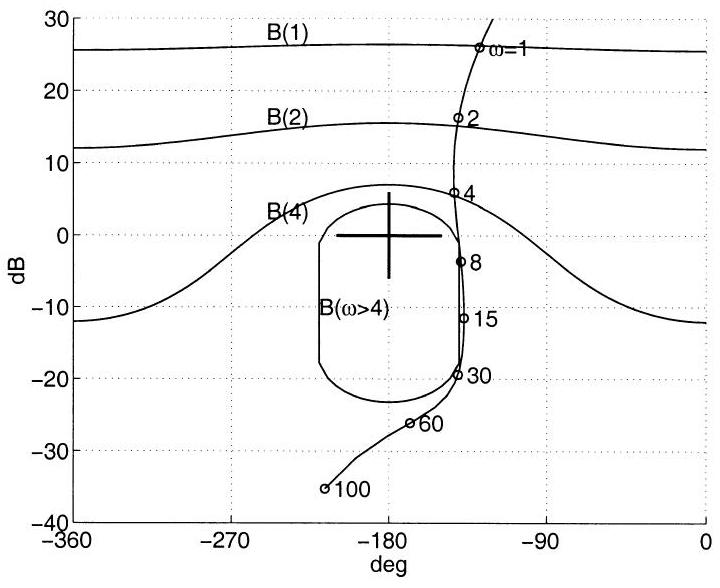
\includegraphics[max width=\textwidth]{2022_07_13_5539d24351f7cdb87589g-51}

Figura 3.6. Límites y $L_{2}=G_{2} P_{0}$

(La ganancia está en el intervalo $[1,2])$. El controlador $G_{3}$ resulta ser:
$$
G_{3}=28 \frac{(1+s / 6)(1+s / 18.6)}{1+s / 14} \frac{39^{2}}{s^{2}+39 s+39^{2}} .
$$
La Fig. $3.8$ muestra los límites de ambas plantas inciertas. Los límites de baja frecuencia son los mismos, pero los límites de alta frecuencia para el caso de incertidumbre expandida son $8 d B$ mayores que para la planta de baja incertidumbre. Como resultado, la ganancia del controlador de alta frecuencia, para la planta de baja incertidumbre, (también la amplitud del controlador y la amplificación del ruido del sensor en la entrada de la planta en altas frecuencias) es de aproximadamente $ 10 \mathrm{~dB}$ menos que la ganancia correspondiente para la planta con gran incertidumbre.

Ejemplo 3: El modelo más simple de un motor de CC cargado con transmisión flexible es:
$$
\begin{aligned}
J_{l} \ddot{\theta}_{l} &=T_{l}-B_{l} \dot{\theta}_{l}+T_{d l} \\
J_{m} \ddot{\theta}_{m} &=T_{m}-B_{m} \dot{\theta}_{m}-T_{l} / n \\
T_{m} &=i k_{t}
\end{aligned}
$$
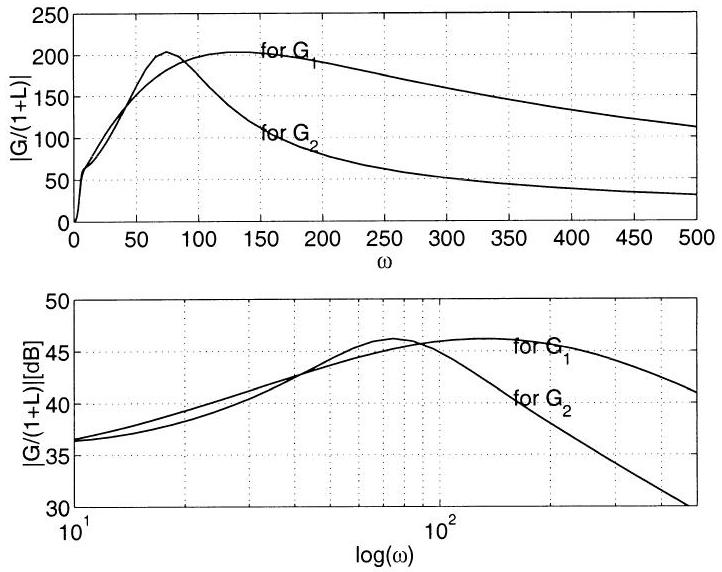
\includegraphics[max width=\textwidth]{2022_07_13_5539d24351f7cdb87589g-52}

Figura 3.7. Comparación de los dos TF desde la salida del sensor hasta la entrada de la planta para los dos diseños $G_{1}$ y $G_{2}$, gráfico superior en escala aritmética, inferior es un diagrama de Bode
$$
T_{l}=\left(\theta_{m} / n-\theta_{l}\right) c_{m l}+\left(\dot{\theta}_{m} / n-\dot{\theta}_{l}\right) d_{m l} .
$$
Los símbolos tienen el siguiente significado:

$i$ - la corriente del motor

$k_{t}$ - la constante e.m.f del motor

$B_{m}$ - la fricción viscosa en el eje del motor

$J_{m}$ - la inercia del motor

$T_{m}$ - el momento eléctrico

$\theta_{m}$ - el ángulo del motor

$n$ - la relación de transmisión

$c_{m l}$ - el factor de resorte de transmisión

$d_{m l}$ - el factor de amortiguación de transmisión

$T_{l}$ - el momento transferido a la carga

$B_{l}$ - la fricción viscosa en la carga

$J_{l}$ - la inercia de carga

$\theta_{l}$ - el ángulo de carga

$T_{d l}$ - el momento de perturbación en la carga.

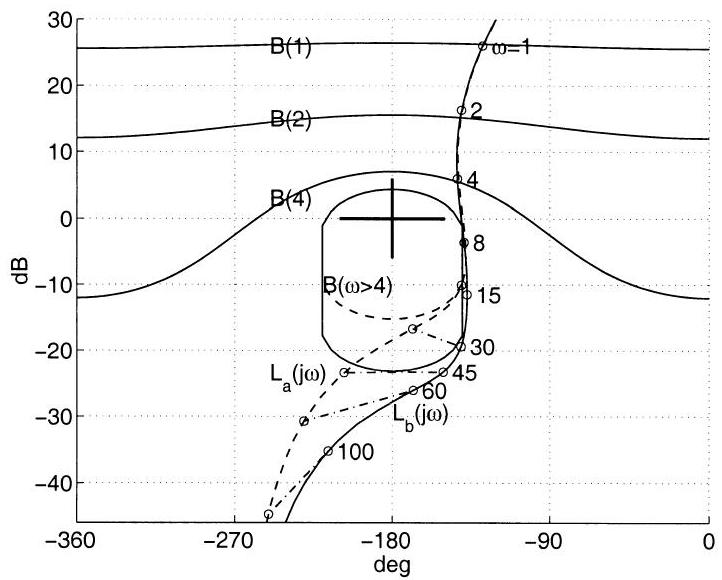
\includegraphics[max width=\textwidth]{2022_07_13_5539d24351f7cdb87589g-53}

Figura 3.8. Comparación de dos diseños: $L_{b}$ para el caso de incertidumbre expandida (límites rígidos), $L_{a}$ para el caso de baja incertidumbre (límites rígidos en bajas frecuencias y límites discontinuos en frecuencias altas)

Si se pueden descuidar $B_{l}$ y $B_{m}$, los TF del comando actual, $i$, al ángulo del motor, $\theta_{m}$, y el ángulo de carga, $\theta_{l}$, son:
$$
\begin{aligned}
&\frac{\theta_{m}}{i}=\frac{k_{t} J_{l}\left(s^{2}+\frac{d_{m l}}{J_{l}} s+\frac{c_{m l}}{J_{l}}\right)}{J_{m} J_{l} s^{2}\left(s^{2}+\left(\frac{d_{m l}}{J_{l}}+\frac{d_{m l}}{n^{2} J_{m}}\right) s+\frac{c_{m l}}{J_{l}}+\frac{c_{m l}}{n^{2} J_{m}}\right)} \\
&\frac{\theta_{l}}{i}=\frac{k_{t}\left(c_{m l}+d_{m l} s\right)}{n J_{m} J_{l} s^{2}\left(s^{2}+\left(\frac{d_{m l}}{J_{l}}+\frac{d_{m l}}{n^{2} J_{m}}\right) s+\frac{c_{m l}}{J_{l}}+\frac{c_{m l}}{n^{2} J_{m}}\right)} .
\end{aligned}
$$
Para la planta descrita anteriormente para $\theta_{m} / i$, asumimos los siguientes valores numéricos: $d_{m l} / J_{l}=2, c_{m l} / J_{l}=100, d_{m l} / J_{m}=0.4, c_{m l} / J_{m}=20, n=1$, $k_{t} / J_{m}=1$. Se supone que la incertidumbre sólo actúa sobre la carga, $J_{l}$, que puede ser hasta 5 veces su valor nominal. Se requiere un controlador tal que $(i)$ el bucle cerrado sea estable; (ii) a frecuencias entre $[1,2] \mathrm{rad} / \mathrm{sec}$, la sensibilidad es menor que $[-20,-7] d B$, respectivamente; y iii) en todas las frecuencias de ganancia y márgenes de fase del formulario $1 /|1+L|<3.5 d B$ are satisfied. Ejemplos de tales sistemas se muestran en la Fig. 3.9. Tenga en cuenta el cambio en los límites cerca de la frecuencia de resonancia, como resultado de la gran incertidumbre de la planta cerca de la frecuencia de resonancia. El controlador resultante es:
$$
G_{1}=22 \frac{(1+s / 3)(1+s / 76)}{1+s / 15} \frac{95^{2}}{s^{2}+150 s+95^{2}}
$$
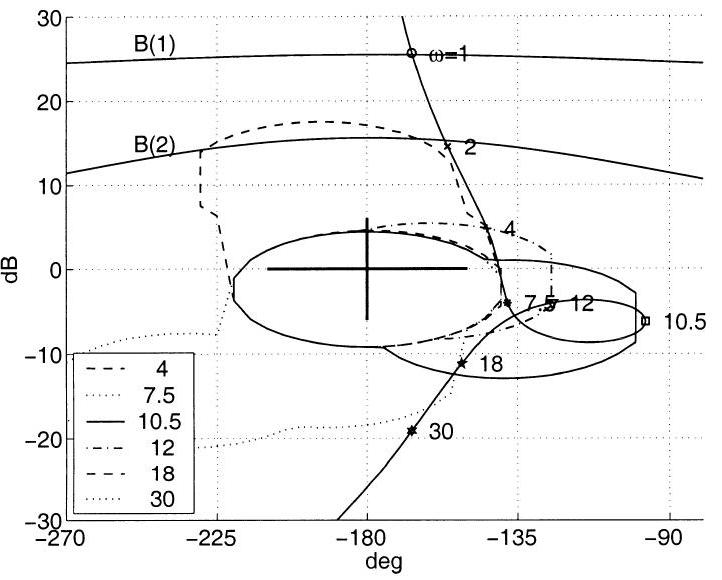
\includegraphics[max width=\textwidth]{2022_07_13_5539d24351f7cdb87589g-54}

Figura 3.9. Límites y bucle abierto para el ejemplo 3

Ejemplo 4: El objetivo de este ejemplo es demostrar cómo QFT maneja plantas inciertas con poca humedad. La planta fue sugerida por primera vez por Wie y Byun (1987). Puede representar un modelo de un motor de CC cargado cuyo sensor se encuentra en la carga misma (ver ecuación (3.4) para muy pequeño $d_{m l}$ )
$$
\{P\}=\frac{k}{s^{2}\left(s^{2}+0.2 \sqrt{2 k} s+2 k\right)}, k \in[0.5,2] .
$$
Se requiere un diseño de controlador tal que, para cualquier planta en $\{P\}$ : i) el circuito cerrado es estable, (ii) en todas las frecuencias ganancia y márgenes de fase de la forma $\mid 1+$ $\left. L(j \omega)\right|^{-1}<6 d B$ are satisfied; and (iii) the cross-over frequency is the highest possible but less than the resonance frequency. La motivación para usar la especificación (iii) es limitar el esfuerzo de control, ya que aumenta rápidamente para frecuencias cruzadas para las cuales la fase de la planta es mucho menor que $ 180^{\circ}$.

Las curvas delimitadoras y el diseño correspondiente se muestran en la Fig. $3.10$ donde se elige la planta nominal para ser $k=0.5$. Cada subgráfico contiene un solo límite junto con la respuesta de bucle nominal y una sola frecuencia. Dado que el bucle abierto casi toca su curva límite por debajo de la frecuencia de cruce, se considera un diseño eficiente. Tratar de aumentar la frecuencia de cruce aumentará enormemente el ancho de banda (ver ejercicio 3.6). El controlador es:
$$
G=0.14 \frac{s^{2} / 0.01+0.16 / 0.01 s+1}{(1+s / 5)(1+s / 0.6)(1+s / 0.04)} .
$$
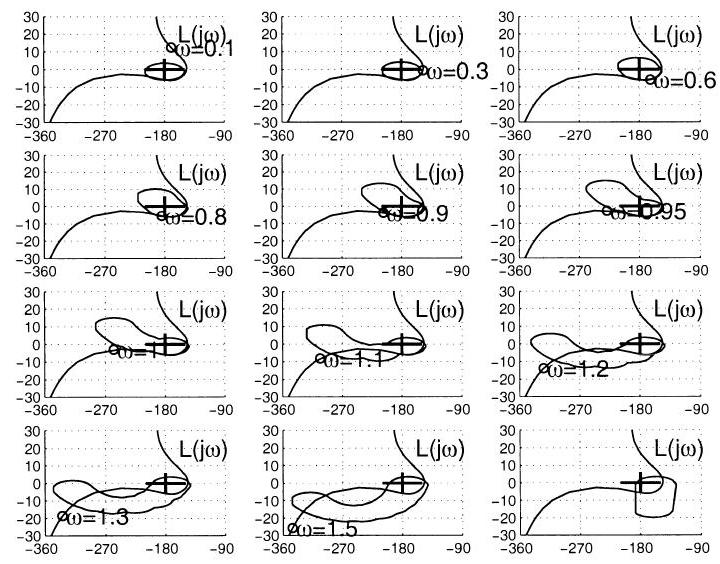
\includegraphics[max width=\textwidth]{2022_07_13_5539d24351f7cdb87589g-55}

Figura 3.10. Límites y transmisión de bucle para $L_{1}=G_{1} P_{0}$ - cada subgráfica representa la transmisión de bucle y los límites a una sola frecuencia (denotada por ow $=f r e q u e n c y$ en la curva delimitadora)

\section{DOS SISTEMAS DOF}
El sistema de retroalimentación de interés se representa esquemáticamente en la Fig. 3.11, y se describe matemáticamente mediante las ecuaciones:
$$
\begin{aligned}
y &=P u \\
u &=-G H y+G F r .
\end{aligned}
$$
Nuestra preocupación es cómo diseñar un controlador, $G(s)$, y prefiltrar, $F(s)$, de tal manera que

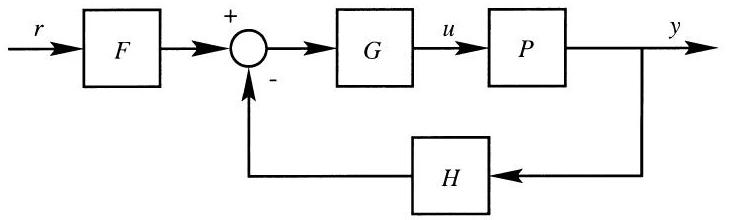
\includegraphics[max width=\textwidth]{2022_07_13_5539d24351f7cdb87589g-56}

Figura 3.11. Un sistema de retroalimentación de dos DOF

para un conjunto dado de plantas, $\{P\}$, el circuito cerrado es estable y se cumplen ciertas especificaciones de dominio $\omega$. Las especificaciones de $\omega$-domain son de los dos tipos siguientes:

(i) coincidencia de modelos: para un conjunto de plantas dado, $\{P\}$, y un TF $F_{m}(s)$
$$
\left|\frac{P G F(j \omega)}{1+L(j \omega)}-F_{m}(j \omega)\right| \leq \delta_{m}(\omega), \forall P \in\{P\}
$$
ii) seguimiento - para un conjunto de plantas dado, $\{P\}$,
$$
\alpha(\omega) \leq\left|\frac{P G F(j \omega)}{1+L(j \omega)}\right| \leq \beta(\omega), \forall P \in\{P\} .
$$
La especificación de coincidencia de modelos limita la distancia de $F_{m}(s)$, el $\mathrm{TF}$ deseado del TF de seguimiento en $\delta_{m}(\omega)$, mientras que la especificación de seguimiento coloca límites superior e inferior, $\beta(\omega)$ y $\alpha(\omega)$ respectivamente, en la amplitud del TF de seguimiento.

El problema de coincidencia de modelos se puede reducir al problema de sensibilidad descrito en la sección 2. Si permitimos $F \equiv H F_{m}$, entonces la desigualdad (3.5) se convierte en:
$$
\left|\frac{F_{m}(j \omega)}{1+L(j \omega)}\right| \leq \delta_{m}(\omega), \forall P \in\{P\} .
$$
La especificación de seguimiento se divide entre la tarea del controlador, $G$, y la del prefiltro, $F$. El trabajo del controlador es reducir la diferencia entre las salidas mínimas y máximas de la planta, $y_{\min }$ y $y_{\max }$ (en una escala logarítmica), debido a la incertidumbre de la planta, mientras que al mismo tiempo garantiza la estabilidad del circuito cerrado. La tarea principal de $F$, por otro lado, es desplazar los diagramas de Bode de $P G /(1+P G$ ) (en una escala $\log$), para que estén dentro de los límites de la especificación. Esto se muestra gráficamente en la Fig. 3.12. El efecto de $F$ y $G$ se explicará en la secuela.

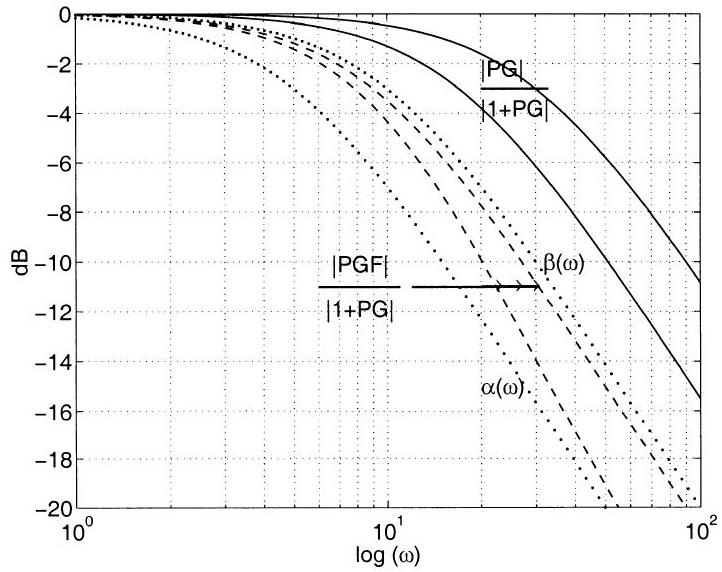
\includegraphics[max width=\textwidth]{2022_07_13_5539d24351f7cdb87589g-57}

Figura 3.12. Diferentes efectos de $G$ y $F$ en el circuito cerrado TF: La respuesta de $\mid P G /(1+$ $P G) \mid$ se sitúa entre las dos líneas sólidas superiores, debido a la incertidumbre de la planta. Las especificaciones requeridas para la respuesta de bucle cerrado son las dos líneas punteadas. El filtro $F$ da forma a las dos líneas sólidas superiores para que caigan dentro de las especificaciones (líneas discontinuas).

El $\mathrm{TF}, F(s)$, es una solución a la desigualdad (3.6) si y sólo si satisface las desigualdades:
$$
\begin{aligned}
&\log \alpha(\omega)-\min _{P \in\{P\}} \log \left|\frac{P G(j \omega)}{1+L(j \omega)}\right| \leq \log | F(j \omega)|, \text { y } \\
&\log \beta(\omega)-\max _{P \in\{P\}} \log \left|\frac{P G(j \omega)}{1+L(j \omega)}\right| \geq \log | F(j \omega)| .
\end{aligned}
$$
Cabe señalar que para una función de amplitud dada $ | A(\omega)|$, siempre existe un TF de fase mínima estable, $F(s)$, tal que $| A(\omega)|=| F(j \omega)|$ (Horowitz 1963). Esto a su vez implica la existencia de una solución de fase mínima, $F(s)$, si se mantiene la siguiente desigualdad
$$
\max _{P \in\{P\}} \log \left|\frac{P G(j \omega)}{1+L(j \omega)}\right|-\min _{P \in\{P\}} \log \left|\frac{P G(j \omega)}{1+L(j \omega)}\right| \leq \log \frac{\beta(\omega)}{\alpha(\omega)} .
$$
Nótese que la desigualdad (3.8) depende solo de $G(s)$ y de la incertidumbre de la planta. El trabajo, por lo tanto, del controlador, es reducir la incertidumbre del bucle cerrado el filtro $F$ no contribuye a este fin. El prefiltro, $F$, simplemente posiciona el $P G /(1+L)$, para todos los $P \in\{P\}$, para que se encuentren dentro de las curvas especificadas, pero no cambia la incertidumbre de $P G F /(1+P G F)$ en una escala logarítmica.

\subsection{CÁLCULO DE LÍMITES}
Ahora se presentan dos algoritmos adicionales para calcular límites en $G(s)$. El primero se basa en la noción de "plantillas" y su principal ventaja es la excelente visión que proporciona sobre las relaciones entre la incertidumbre de la planta, las especificaciones de bucle cerrado, el ancho de banda, la programación y la estructura del controlador. El segundo de los dos es un algoritmo de forma cerrada, que se recomienda cuando el número discreto de plantas en $\{P\}$ es pequeño. De aquí en adelante asumiremos, sin pérdida de generalidad, que $H \equiv 1$.

\subsection{CÁLCULOS DE LÍMITES CON LA AYUDA DE PLANTILLAS DE PLANTA}
Un TF, $P(s)$, evaluado a una frecuencia dada, $\omega$, es un número complejo, el conjunto de todos los números complejos para un conjunto dado de TF, $\{P\}$, evaluado a una frecuencia dada $\omega$, es decir,
$$
T_{\omega}=\{P(j \omega) \mid P \in\{P\}\},
$$
se denomina la plantilla de $\{P\}$ en $\omega$. La región etiquetada 'A' en el gráfico de Nichols de la Fig. 3.13, describe la plantilla de $\{P\}=k / s(s+a)$ para $k \in[1,5]$ y $a \in[1,2]$ a la frecuencia de $\omega=1 \mathrm{rad} / \mathrm{sec}$. Los valores de bucle cerrado para esta plantilla, es decir, la intersección de los extremos de la plantilla con las curvas $P G /(1+P G)$ en el gráfico de Nichols, para todos los $P \in T_{\omega}$, van desde $-6 d B$ a $3 d B$. Por lo tanto, para $G=1$ (plantilla A), la incertidumbre del bucle cerrado es:

$20 \log \max _{P \in\{P\}}\left|\frac{P(j \omega)}{1+P(j \omega)}\right|-20 \log \min _{P \in\{P\}}\left|\frac{P(j \omega)}{1+P(j \omega)}\right|=3-(-6)=9 d B .$

La plantilla para $\{P G\}$ tiene la misma forma que la plantilla $\{P\}$, pero se encuentra $20 \log | G(j \omega)|$ encima y $\arg G(j \omega)$ grados a la derecha. La Fig. $3.13$ incluye dos ejemplos, la plantilla para $G=\left[16 d B, 0^{\circ}\right]$ etiquetada ' ${ }^{\prime}$ ' y para $G=\left[19 d B, 50^{\circ}\right]$ labeled ' $\mathrm{C}$ '. Simplemente deslizando la plantilla en el gráfico de Nichols, una lectura de la cantidad de incertidumbre que el circuito cerrado

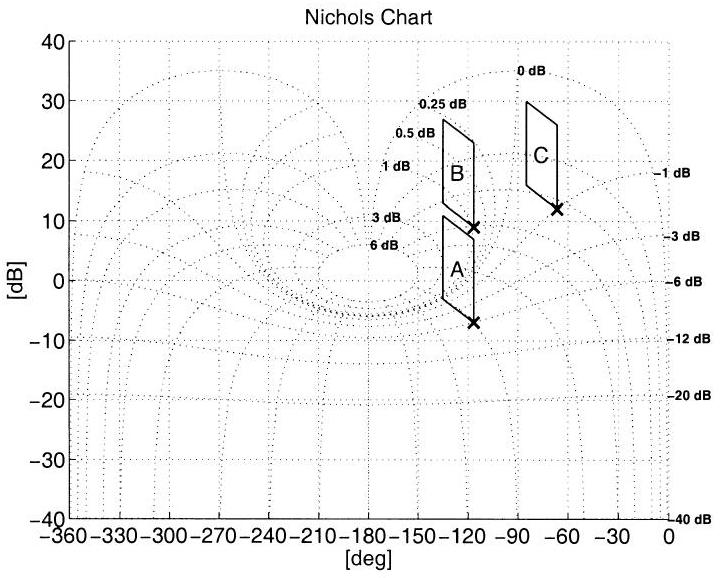
\includegraphics[max width=\textwidth]{2022_07_13_5539d24351f7cdb87589g-59}

Figura 3.13. Las plantillas para $\omega=1 \mathrm{rad} / \mathrm{sec}$ consisten en todos los números complejos dentro de la curva cerrada ' $\mathrm{A}$ '; ' $\mathrm{B}$ ' es la misma plantilla pero desplazada por $16 d \mathrm{~B} ;$ ' $\mathrm{C}$ ' se desplaza por $19 \mathrm{~dB}$ y $50^{\circ}$. El símbolo $\times$ en la esquina inferior derecha de todas las plantillas indica la planta nominal

$\frac{P G(j \omega)}{1+P G(j \omega)}$ puede tolerar, se puede obtener fácilmente. Para una fase dada de $G(j \omega)$, siempre existe una amplitud mínima de $G(j \omega)$ por encima de la cual la incertidumbre de bucle cerrado de $\left|\frac{P G(j \omega)}{1+P G(j \omega)}\right|$ es menor que un valor deseado. El procedimiento de cálculo consolidado para un conjunto de frecuencias $\omega \in \Omega$ y especificaciones dadas en la forma $\alpha, \beta$, será entonces el siguiente:

\begin{enumerate}
  \item Elija una frecuencia $\omega \in \Omega$.

  \item Traza la curva de la plantilla $T_{\omega}$ de $\{P\}$ en un gráfico de Nichols (para un algoritmo eficiente ver Ballance y Hughes (1996)).

  \item Elija arbitrariamente una sola planta $P_{0}(j \omega)$ desde $\{P\}$, designarla como planta nominal y marcar su ubicación en la plantilla.

  \item Discretiza la fase del controlador $\phi$ en pasos de, por ejemplo $\Phi=\{0,-5, \cdots,-360\}$

  \item Elija una sola fase $\phi \in \Phi$. 6. Cambie la plantilla horizontalmente en $\phi^{\circ}$, y luego verticalmente en $z d B$ (ganancia de bucle abierto) sin cambiar la actitud de la plantilla, hasta el punto en que la incertidumbre del bucle cerrado de la plantilla cumpla con la especificación, es decir, el punto donde

\end{enumerate}
$$
\begin{aligned}
20 \log \max _{P \in\{P\}}\left|\frac{P G(j \omega)}{1+P G(j \omega)}\right| &-20 \log \min _{P \in\{P\}}\left|\frac{P G(j \omega)}{1+P G(j \omega)}\right| \\
&=20 \log \frac{\beta(\omega)}{\alpha(\omega)} .
\end{aligned}
$$
Marque la ubicación del punto nominal de la plantilla en el gráfico de Nichols (desplazado por $\phi^{\circ}$ y $z d B$ ). El significado de este punto es que si $\arg G(j \omega)=$ $\phi^{\circ}$ y $| G(j \omega)|>z d B$ (bucle abierto), se satisface la incertidumbre del bucle cerrado en $\omega$, es decir,
$$
\begin{aligned}
20 \log \max _{P \in\{P\}}\left|\frac{P G(j \omega)}{1+P G(j \omega)}\right| &-20 \log \min _{P \in\{P\}}\left|\frac{P G(j \omega)}{1+P G(j \omega)}\right| \\
& \leq 20 \log \frac{\beta(\omega)}{\alpha(\omega)} .
\end{aligned}
$$

\begin{enumerate}
  \setcounter{enumi}{7}
  \item Repita el paso 5 para todos los $\phi \in \Phi$, luego conecte todos los puntos marcados. Esta curva es el límite de $P_{0} G$ a $\omega$; y significa que si $G(s)$ está diseñado de tal manera que $P_{0} G(j \omega)$ se encuentra encima de él, entonces se cumplen las especificaciones de bucle cerrado.

  \item Repita el paso $2-7$ para todas las frecuencias en $\Omega$.

\end{enumerate}
Mientras $\beta(\omega) / \alpha(\omega)$ esté lo suficientemente cerca de 1 , entonces para cada ángulo de fase $\phi \in$ $[0,2 \pi]$ existe una amplitud finita de $G(j \omega)$ por encima de la cual se satisface la incertidumbre del bucle cerrado. El límite será entonces una curva que cruza el gráfico de Nichols desde la derecha $(\phi=0)$ a la izquierda $(\phi=-360)$. Un límite de este tipo se llama límite abierto y las frecuencias para las cuales los límites están abiertos se llaman límites de baja frecuencia.

A altas frecuencias, las especificaciones son solo márgenes de ganancia y fase, es decir,
$$
\left|\frac{P G}{1+P G}\right| \leq \delta_{n}(\omega) \text { or } \frac{1}{|1+P G|} \leq \delta_{s}(\omega),
$$
por algunos $\delta_{n}(\omega)>1$ y/o $\delta_{s}(\omega)>1$. La misma técnica descrita anteriormente se puede usar para encontrar límites, pero para cada ángulo de fase existen dos valores de $| G(j \omega)|, g_{1}$ y $g_{2}\left(g_{1}<g_{2}\right)$ such that the margin specifications are satisfied if $|G(j \omega)| \leq g_{1}$ or if $|G(j \omega)| \geq g_{2}$. La curva delimitadora resultante es cerrada, a menos que la incertidumbre sea demasiado amplia en fase. Un límite de este tipo se denomina límite cerrado y las frecuencias para las cuales los límites son cerrados y mayores que los límites de baja frecuencia se denominan límites de alta frecuencia.

Ejemplo: Dada la planta incierta $\{P\}=\frac{k}{s(s+a)}$ para $k \in[1,5]$ y $a \in[1,2]$ las especificaciones son
$$
\begin{array}{ll}
1=\alpha \leq\left|\frac{P G F(j \omega)}{1+P G(j \omega)}\right| \leq \beta=1.12, \text { for } \omega=1 \\
\left|\frac{P G(j \omega)}{1+P G(j \omega)}\right| \leq 2=6 d B, \text { for } \omega \geq 0 .
\end{array}
$$
El límite abierto, etiquetado $B_{1}$ en la Fig. 3.14, es el límite para $\omega=1 \mathrm{rad} / \mathrm{sec}$. La planta en $\omega=1$ es la inferior con un ' 1 ' en su centro. Al mover la plantilla verticalmente (aumentando la ganancia de bucle abierto en $17 d \mathrm{~dB}$ ), su incertidumbre de bucle cerrado se reduce a $1 d B$ (1.12 en unidades aritméticas). La planta nominal $P_{0}=\frac{1}{s(s+2)}$, marcada en la plantilla por un $\times$, incide en la curva delimitadora $B_{1}$. Lo mismo ocurre cuando la plantilla se desplaza por $18.7 \mathrm{~dB}$ y $50^{\circ}$, (ver la planta en la esquina superior derecha con un ' 1 ' en su centro). La curva de límite cerrado $B_{5}$, en la Fig. 3.14, es el límite para $\omega=5 \mathrm{rad} / \mathrm{sec}$. La plantilla para $\omega=5 \mathrm{rad} / \mathrm{sec}$ es la más baja en el gráfico con un ' 5 ' en su centro. Aumentar su ganancia de bucle abierto en $11 d B$ y cambiarla en $-20^{\circ}$ da como resultado que su incertidumbre de bucle cerrado sea inferior a $6 d B$ (la plantilla no entra en la región de $6 d B$ pero solo la toca) y la planta nominal, $P_{0}=\frac{1}{s(s+2)}$, marcada en la plantilla por un $\times$,  toca la parte inferior de la curva delimitadora cerrada (véase la plantilla marcada ' 5 ' cuyo punto nominal es de aproximadamente $-18 d B)$. Lo mismo ocurre cuando la plantilla se desplaza verticalmente en $35 d B$ (ganancia de bucle abierto) sin cambiar su ángulo de fase (ver la plantilla superior con un $' 5$ ' en su centro en el gráfico). Por lo tanto, para un controlador con un ángulo de fase de $-20^{\circ}$ en $\omega=5 \mathrm{rad} / \mathrm{sec}$, hay dos puntos en la curva delimitadora cerrada que significa: $| G(j 5)|$ debe ser inferior a $11 d B$ o superior a $35 d B$ para satisfacer las especificaciones a $\omega=5$.

\subsection{CÁLCULO DE LÍMITES MEDIANTE UN ALGORITMO DE FORMA CERRADA}
Para una frecuencia dada $\omega$ y dos plantas dicen $P_{1}, P_{2}$, donde $\left|\frac{P_{2} G}{1+P_{2} G}\right|>$ $\left|\frac{P_{1} G}{1+P_{1} G}\right|$, la desigualdad (3.8) se reduce a
$$
\left|\frac{\left(1+P_{1} G\right)}{\left(1+P_{2} G\right)} \frac{P_{2}}{P_{1}}\right| \leq \frac{\beta(\omega)}{\alpha(\omega)}
$$
Si su lado izquierdo es mayor que 1 , de lo contrario se convierte en:
$$
\left|\frac{\left(1+P_{2} G\right)}{\left(1+P_{1} G\right)} \frac{P_{1}}{P_{2}}\right| \leq \frac{\beta(\omega)}{\alpha(\omega)} .
$$
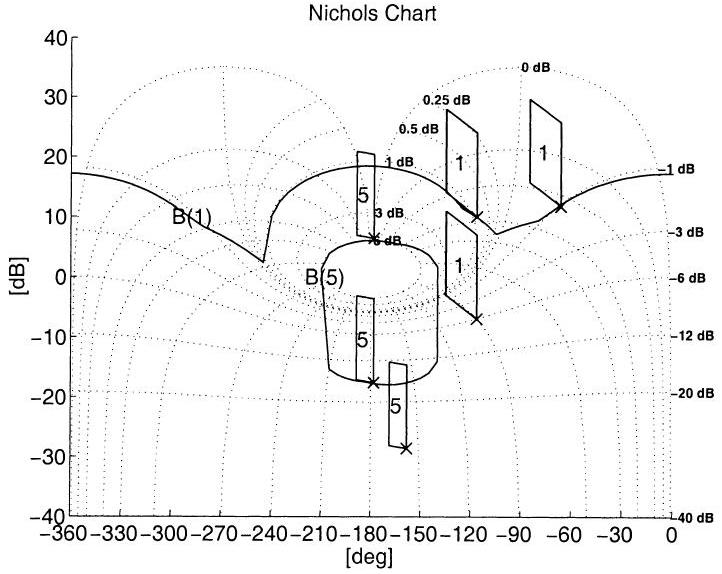
\includegraphics[max width=\textwidth]{2022_07_13_5539d24351f7cdb87589g-62}

Figura 3.14. Plantillas y límites: Para $\omega=1$ la plantilla es la estructura más baja con un ' 1 ' en su centro, las otras plantillas son del mismo tamaño y forma pero desplazadas verticalmente (aumento o disminución de la ganancia del bucle abierto) u horizontalmente (fase de bucle abierto sumada o restada) o ambas. La curva delimitadora $B_{1}$ es un límite abierto. Para $\omega=5$ la plantilla es la más baja con un ' 5 ' en su centro y su curva delimitadora $B_{5}$ es un límite cerrado

Su solución es un círculo en el plano complejo, tal que si $G(j \omega)$ se encuentra en su interior, la desigualdad no se sostiene. Esto se puede ver dejando $G \equiv \infty$, de modo que la desigualdad (3.9) tiende a 1 . Esto implica que la desigualdad es cierta, lo que implica además que $G$ no está en el interior del círculo. El centro y el radio de este círculo pueden calcularse fácilmente por analogía con el procedimiento de la sección 2.3. Dejar
$$
L=\left(1+P_{1} G\right) \frac{P_{2}}{P_{1}-P_{2}}
$$
Da:
$$
\left|\frac{L}{1+L}\right| \leq \frac{\beta}{\alpha}=a,
$$
cuya solución, al parámetro $L$, es el círculo situado en $z_{1}=\left[a^{2} /\left(1-a^{2}\right), 0\right]$ con radio $r_{1}=a /\left|1-a^{2}\right|$ (ver sección 2.3). La solución al parámetro $1+P_{1} G$ será entonces el círculo ubicado en $z_{2}=z_{1}\left(P_{1} / P_{2}-1\right)$ con radio $r_{2}=r_{1}\left| P_{1} / P_{2}-1\right|$. Del mismo modo, la solución al parámetro $P_{1} G$ será el círculo ubicado en $z_{3}=z_{2}-1$ con radio $r_{3}=r_{2}$, y la solución al parámetro $G$ será el círculo ubicado en $z_{4}=z_{3} / P_{1}$ con radio $r_{4}=r_{3} /\left| P_{1}\right|$ que es la solución a la desigualdad (3.9) para el parámetro $G$. Por lo tanto, un algoritmo para encontrar límites en $G(j \omega)$ que resuelva la desigualdad (3.7) será el siguiente:

\begin{enumerate}
  \item Discretiza el conjunto de plantas inciertas en un conjunto finito $\{P\}=\left\{P_{1}, \cdots, P_{n}\right\}$.

  \item Elija dos plantas $P_{i}, P_{j}$ desde $\{P\}$.

  \item Calcula el círculo que resuelve la desigualdad (3.9) para $P_{1}=P_{i}$ y $P_{2}=P_{j}$.

  \item Repita el paso 3 para todos los pares de plantas, $P_{i}, P_{j}$, en $\{P\}$.

  \item La curva formada por la unión de todos los círculos calculados en el paso 4 es el límite $B(\omega)$.

\end{enumerate}
\subsection{UN EJEMPLO}
Conjunto de plantas y especificaciones
$$
\{P\}=\frac{k}{s(s+a)}, k \in[1,10], a \in[1,10] .
$$
Se requiere diseñar un controlador, $G(s)$, y un prefiltro, $F(s)$, de modo que (i) la respuesta de bucle abierto de $L(s)$ satisfaga las especificaciones de margen.
$$
\left|\frac{L(j \omega)}{1+L(j \omega)}\right|<3 d B, \forall \omega \geq 0
$$
y (ii) la amplitud del TF de bucle cerrado de $r$ a $y$ estará limitada entre las siguientes funciones $\beta(\omega)$ y $\alpha(\omega)$

\begin{tabular}{|c|c|c|c|c|c|}
\hline
$\omega$ & $0.5$ & 1 & 2 & 4 & 8 \\
\hline
$\beta(\omega)[d B]$ & 0 & 0 & $-1$ & $-4$ & $-7$ \\
\hline
$\alpha(\omega)[d B]$ & $-0.5$ & $-1$ & $-3$ & $-8$ & $-14$ \\
\hline
\end{tabular}

Diseño del controlador - El conjunto elegido de frecuencias, $\Omega$, es el conjunto para el que se dan las especificaciones de seguimiento e incluye las frecuencias altas $15,30,60$, 100 y 200. Los límites se muestran en la Fig. $3.15$ para la planta nominal $\frac{1}{s(s+1)}$, que también incluye la transmisión de bucle con forma para el controlador
$$
G=\frac{52(1+s / 70)(1+s / 6)}{(1+s / 0.3)\left(s^{2} / 170^{2}+s / 170+1\right)} .
$$
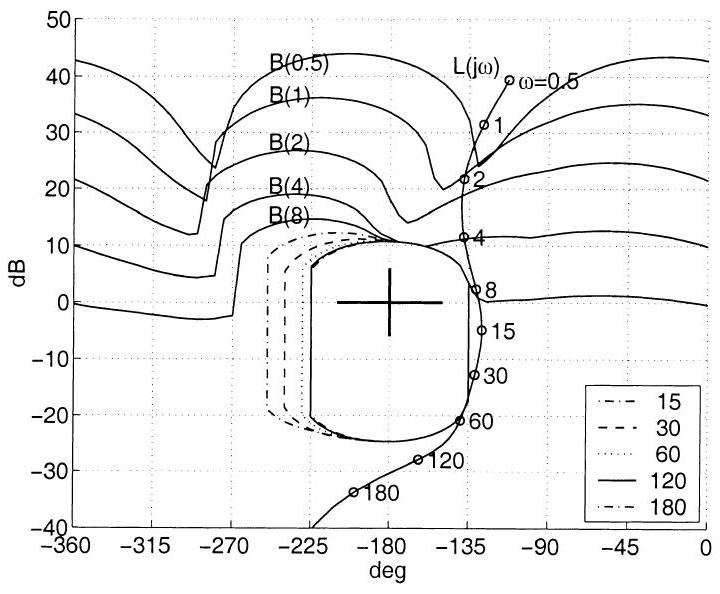
\includegraphics[max width=\textwidth]{2022_07_13_5539d24351f7cdb87589g-64}

Figura 3.15. Límites y bucle abierto

Diseño del prefiltro - Se simuló la amplitud del TF $\frac{P G(j \omega)}{1+P G(j \omega)}$ para 100 plantas (para cada entero en el rango de $k^{\prime} s$ y $a^{\prime} s$ ). Los valores máximos y mínimos en las frecuencias de especificación de seguimiento se muestran en la Fig. 3.16, línea rígida, que también incluyen las especificaciones y el bucle cerrado máximo y mínimo de amplitud, $\left|\frac{P G F(j \omega)}{1+P G(j \omega)}\right|$, utilizando el prefiltro
$$
F=\frac{\left(s^{2}+11.2 s+64\right) / 64}{(1+s / 2.8)(1+s / 8)(1+s / 35)},
$$
Claramente las especificaciones están satisfechas.

\section{EXTENSIÓN A PLANTAS NMP}
Los tipos de plantas NMP abordados aquí son plantas con retardo puro y/o ceros RHP incrustados en una estructura de retroalimentación (Fig. $3.1$ o Fig. 3.11). Por lo tanto, su transmisión de bucle, $L=P G$, tiene un ancho de banda limitado, es decir, existe un $\omega$ tal que $L(j \omega)=0 d B$, donde $\omega$ disminuye a medida que disminuyen los ceros RHP o el retraso aumenta (ver Capítulo 2). La técnica de diseño descrita en las secciones anteriores también es adecuada para plantas de NMP, pero pueden surgir dificultades.

\includegraphics[max width=\textwidth]{2022_07_13_5539d24351f7cdb87589g-65}

Figura 3.16. Diseño del prefiltro: Las líneas rígidas son máximo y mínimo de $| P G /(1+P G)|$, las líneas discontinuas son máximo y mínimo de $| P G F /(1+P G)|$, los signos $+$ son las especificaciones $\beta(\omega)$ y $\alpha(\omega)$ respectivamente

debido a las limitaciones de ancho de banda, que son: i) en el caso de las instalaciones estables, los requisitos contradictorios de gran ancho de banda para las especificaciones de bucle cerrado «ajustados» y las limitaciones máximas de anchura de banda debidas a ceros y retrasos de RHP; y ii) para las plantas inestables, los requisitos contradictorios de gran ancho de banda para especificaciones de bucle cerrado "ajustados", las limitaciones mínimas de ancho de banda debidas a los polos RHP y las limitaciones máximas de ancho de banda debidas a ceros y retrasos de RHP. Las plantas que incluyen polos RHP y ceros (o retrasos) pueden tener serias limitaciones de circuito cerrado, especialmente limitaciones de ganancia y margen de fase. Para una discusión cuantitativa ver Horowitz (1979).

Un argumento cuantitativo, basado en la transformada de Hilbert, se describe ahora para reforzar una explicación pictórica del fenómeno de limitación del rendimiento de bucle cerrado NMP. Dejando $L_{M}(s)$ denota una TF estable y de fase mínima, las integrales de Bode (Horowitz 1963) relacionan su fase, $\arg \left(L_{M}(j \omega)\right)$, a su amplitud, $\log \left| L_{M}(j \omega)\right|$, vienen dadas por la ecuación integral principal:
$$
\arg L_{M}\left(j \omega_{0}\right)=\frac{1}{\pi} \int_{0}^{\infty} \frac{d \log L_{M}(j \omega)}{d u} W(u) d u \text {, where }
$$
$$
u=\log \frac{\omega}{\omega_{0}}, W(u)=\log \left(\operatorname{coth} \frac{|u|} {2}\right)=\log \frac{\omega+\omega_{0}}{\omega-\omega_{0}} .
$$
La función de ponderación $W(u)$ es infinita en $\omega_{0}$, muy grande en la vecindad de $\omega_{0}$ y disminuye con $\left|\omega-\omega_{0}\right|$, es decir, está cerca de la función $\delta\left(\omega-\omega_{0}\right)$. Por lo tanto, en promedio para un intervalo de frecuencia suficientemente grande podemos concluir que: la fase de $L_{M}(j \omega)$ (que es negativa) es mayor (más cercana a cero) si la pendiente de la amplitud de $L_{M}(j \omega)$ en la escala $\log$ (que es negativa) es mayor (más cercana a cero). Además, si su fase es positiva (negativa), entonces su amplitud es una función creciente (decreciente) de $\omega$. Esta observación es cierta en promedio en intervalos de frecuencia suficientemente grandes, pero como la fase de $L_{M}(j \omega)$ tiende a cero, se vuelve casi puntual. La prueba y las condiciones bajo las cuales esto es cierto siguen.

Supongamos que $\arg L_{M}(j \omega) \leq 0$ para todas las frecuencias excepto para aquellas dentro del intervalo $\left[\omega_{1}, \omega_{2}\right]$ donde $\arg L_{M}(j \omega)>0$. Uso de la transformada de Hilbert
$$
\log \left| L_{M}\left(j \omega_{0}\right)\right|=\frac{2}{\pi} \int_{0}^{\infty} \frac{\omega \arg L_{M}(j \omega)}{\omega_{0}^{2}-\omega^{2}} d w,
$$
Se puede demostrar fácilmente que
$$
\begin{aligned}
\log \frac{L_{M}\left(j \omega_{1}\right)}{L_{M}\left(j \omega_{2}\right)} &=\log L_{M}\left(j \omega_{1}\right)-\log L_{M}\left(j \omega_{2}\right) \\
&=\frac{2}{\pi} \int_{0}^{\infty} \frac{\left(\omega_{2}^{2}-\omega_{1}^{2}\right) \omega}{\left(\omega_{1}^{2}-\omega^{2}\right)\left(\omega_{2}^{2}-\omega^{2}\right)} \arg L_{M}(j \omega) d w
\end{aligned}
$$
que es negativo porque el signo de $\arg L_{M}(j \omega)$ es positivo en $\left[\omega_{1}, \omega_{2}\right]$ y negativo en los intervalos $\left(0, \omega_{1}\right)$, y $\left(\omega_{2}, \infty\right)$. Esto se muestra en la Fig. 3.17. Así, como $\arg L_{M}(j \omega) \rightarrow 0$ en el intervalo $\left[\omega_{1}, \omega_{2}\right],\left| L_{M}\left(j \omega_{2}\right)\right| \geq\left| L_{M}\left(j \omega_{1}\right)\right|^{1}$.

Las observaciones anteriores nos ayudarán a comprender el fenómeno NMP del siguiente ejemplo. La Fig. $3.18$ muestra una transmisión de bucle, $L_{0}=P_{0} G$, para la planta NMP
$$
\{P\}=\frac{k}{s} \frac{20-s}{20+s}, k \in[1,3]
$$
con especificaciones de margen de la forma $1 /|1+L(j \omega)|<3.5$. La Fig. $3.18$ muestra no solo
$$
L_{0}=\frac{20-s}{s+20} \frac{1}{s} G
$$
${ }^{1}$ Se supone que $L_{M}$ es continuo en el intervalo $\left[\omega_{1}, \omega_{2}\right]$\\

\includegraphics[max width=\textwidth]{2022_07_13_5539d24351f7cdb87589g-67}

Figura 3.17. Las figuras etiquetadas (a) y (b) muestran dos trayectorias de una planta de fase mínima en un gráfico de Nichols. La trayectoria de la figura (a) no es factible matemáticamente, mientras que la de la figura (b) sí lo es. Tenga en cuenta que $\omega_{1} \leq \omega_{2}$\\

\includegraphics[max width=\textwidth]{2022_07_13_5539d24351f7cdb87589g-67(1)}

Figura 3.18. Dos NMP TF $L(j \omega)$ y sus partes de fase mínima $L_{M}$ : la ganancia de baja frecuencia de la figura de la derecha es $1.5 d B$ más que la de la izquierda, pero el costo de control en términos de amplitud está aumentando, por ejemplo, $G(j \omega)$ ha aumentado en al menos $10 d B$ a $\omega>300$, pero también su parte de fase mínima,  $L_{M}=\frac{1}{s} G(s)$, para dos diseños. Claramente, cuando uno intenta aumentar el ancho de banda de bucle abierto, sucede lo siguiente: (i) la frecuencia del margen de ganancia aumenta (en este ejemplo de 70 a 300), (ii) el intervalo de frecuencias cercanas al aumento de frecuencias del margen, y (iii) la fase de la fase mínima de la parte de la transmisión de bucle se aproxima a cero y, por lo tanto, no puede reducirse para lograr un mayor margen de ganancia. El resultado es la limitación del ancho de banda.

En el ejemplo anterior, los límites de alta frecuencia son una curva cerrada, debido a la elección de la planta nominal como un sistema NMP. Si la planta nominal se elige como fase mínima, los límites de alta frecuencia se moverán hacia la derecha. El ancho de banda estará limitado por la capacidad de dar forma al bucle de tal manera que rodee los límites desde la derecha. De lo contrario, los límites se rodearán desde la izquierda, lo que significa, según el criterio de estabilidad de Nyquist, que el bucle cerrado, con bucle abierto $L(s)$, es inestable. Este cerco debe tener lugar cuando la fase de $L_{M}(j \omega)$ es negativa y siempre que $L_{M}(j \omega)$ pasa cerca de los límites. De lo contrario, según la discusión anterior, la amplitud de $L_{M}(j \omega)$ será una función creciente de $\omega$ y, por lo tanto, no rodeará los límites desde la derecha.

\section{EXTENSIÓN A SISTEMAS DE DATOS MUESTREADOS}
El sistema de retroalimentación tratado se representa esquemáticamente en la Fig. $3.20$ donde $T$ denota el tiempo de muestreo del convertidor A/D $\left(\omega_{s}=2 \pi / T\right.$ es la frecuencia de muestreo) y $*$ significa una señal muestreada tal que
$$
x^{*}(t)=\sum_{k=0}^{\infty} x(k T) \delta(t-k T) .
$$
La transformada de Laplace de esta secuencia es
$$
X^{*}(s)=\sum_{k=0}^{\infty} x(k T) e^{-s k T},
$$
mientras que si $X(s)$ tiene más polos que ceros (Astrom y Wittenmark (1996) p. 280)
$$
X^{*}(s)=\frac{1}{T} \sum_{0}^{\infty} X\left(s-j k \omega_{s}\right) .
$$
El convertidor D/A es un $\mathrm{ZOH}$. Matemáticamente el sistema se describe mediante las ecuaciones $\left(P_{z o h}(z)\right.$ denota el TF de la entrada $\mathrm{ZOH}$ a la salida de $P$ donde $\left.z=e^{s T}\right)$
$$
\begin{aligned}
y &=P_{z o h} u^{*}+d \\
u^{*} &=-G(z)\left(H(z) y^{*}+n^{*}-F(z) r^{*}\right)
\end{aligned}
$$
\includegraphics[max width=\textwidth]{2022_07_13_5539d24351f7cdb87589g-69}

Figura 3.19. Una planta NMP, el bucle abierto nominal, $L_{M}(s)$, es la fase mínima, por lo tanto, los límites se mueven con frecuencia hacia la derecha. Cerca de $\omega=30$, la fase de $L(j \omega)$ debe ser negativa para que su amplitud sea una función decreciente de $\omega$, y por lo tanto los límites estarán rodeados por $L(j \omega)$ desde la derecha, lo que significa que se cumple el criterio de estabilidad de Nyquist.

\includegraphics[max width=\textwidth]{2022_07_13_5539d24351f7cdb87589g-69(1)}

Figura 3.20. Dos sistemas de control de datos muestreados DOF, la salida muestreada $y^{*}$ y la entrada muestreada $u^{*}$ son
$$
\begin{aligned}
y^{*}(s) &=\frac{d^{*}-P_{z o h}^{*} G(z) n^{*}+P_{z o h}^{*} G(z) F(z) r^{*}}{1+P_{z o h}^{*} G(z) H(z)} \\
u^{*}(s) &=\frac{-G(z) H(z) d^{*}-G(z) n^{*}+G(z) F(z) r^{*}}{1+P_{z o h}^{*} G(z) H(z)}
\end{aligned}
$$
Ahora veamos las siguientes especificaciones de circuito cerrado:

\begin{enumerate}
  \item Problema de reducción de sensibilidad: para todos los $P \in\{P\}$ el TF de la perturbación en la salida de la planta a la salida de la planta está limitado por
\end{enumerate}
$$
\left|\frac{y^{*}(z)}{d^{*}(z)}\right|=\left|\frac{1}{1+P_{z o h}^{*} G(z) H(z)}\right|_{z=e^{j \omega T}} \leq \delta_{s}(\omega) .
$$

\begin{enumerate}
  \setcounter{enumi}{2}
  \item Problema de coincidencia de modelo (dado $F_{m}(z)$ ): para todos los $P \in\{P\}$ la distancia del TF desde la entrada de comandos $r^{*}$ a la salida de la planta desde el TF óptimo, $F_{m}(z)$, está limitada por
\end{enumerate}
$$
\left|\frac{y^{*}(z)}{r^{*}(z)}-F_{m}(z)\right|=\left|\frac{P_{z o h}^{*} G(z) F(z)}{1+P_{z o h}^{*} G(z) H(z)}-F_{m}(z)\right|_{z=e^{j \omega T}} \leq \delta_{m}(\omega) .
$$

\begin{enumerate}
  \setcounter{enumi}{3}
  \item Problema de seguimiento: para todos los $P \in\{P\}$ la amplitud del TF desde la entrada de comandos $r^{*}$ hasta la salida de la planta está limitada por
\end{enumerate}
$$
\alpha(\omega) \leq\left|\frac{y^{*}(z)}{r^{*}(z)}\right|=\left|\frac{P_{z o h}^{*} G(z) F(z)}{1+P_{z o h}^{*} G(z) H(z)}\right|_{z=e^{j \omega T}} \leq \beta(\omega) .
$$

\begin{enumerate}
  \setcounter{enumi}{4}
  \item Problema de esfuerzo de control: para todos los $P \in\{P\}$ el TF desde la salida del sensor hasta la entrada de la planta está limitado por
\end{enumerate}
$$
\left|\frac{u^{*}(z)}{n^{*}(z)}\right|=\left|\frac{G(z)}{1+P_{z o h}^{*} G(z) H(z)}\right|_{z=e^{j \omega T}} \leq \delta_{c}(\omega) .
$$
Todas estas especificaciones son equivalentes a las discutidas para sistemas continuos. Por lo tanto, los límites para cada frecuencia, $\omega$, se calculan exactamente como para el caso continuo. La única diferencia es que el controlador, $G(z)$, es discreto, pero en la práctica es lo mismo que dar forma a un controlador continuo. En la caja de herramientas QFT de Matlab ${ }^{\mathrm{TM}}$ (Borghesani et al. (1994)) el diseñador da forma a TF discretos basándose en sus habilidades para dar forma a TF continuos. La idea es la siguiente: El diseñador decide agregar un polo, cero, etc. a la transmisión de bucle, el software elige una aproximación discreta del polo elegido, cero, etc. y muestra una gráfica de Nichols del diseño discreto usando la transformación $z=e^{s T}$. Cuando el diseñador está 	satisfecho con la conformación (que es un criterio pictórico), el controlador discreto ya está disponible sin necesidad de utilizar transformaciones de ningún tipo del dominio continuo al discreto.


%\end{document}